%%%%%%%%%%%%%%%%%%%%%%%%%%%%%%%%%%%%%%%%%
% Masters/Doctoral Thesis 
% LaTeX Template
% Version 2.5 (27/8/17)
%
% This template was downloaded from:
% http://www.LaTeXTemplates.com
%
% Version 2.x major modifications by:
% Vel (vel@latextemplates.com)
%
% This template is based on a template by:
% Steve Gunn (http://users.ecs.soton.ac.uk/srg/softwaretools/document/templates/)
% Sunil Patel (http://www.sunilpatel.co.uk/thesis-template/)
%
% Template license:
% CC BY-NC-SA 3.0 (http://creativecommons.org/licenses/by-nc-sa/3.0/)
%
%%%%%%%%%%%%%%%%%%%%%%%%%%%%%%%%%%%%%%%%%

%----------------------------------------------------------------------------------------
%	PACKAGES AND OTHER DOCUMENT CONFIGURATIONS
%----------------------------------------------------------------------------------------

\documentclass[
11pt, % The default document font size, options: 10pt, 11pt, 12pt
%oneside, % Two side (alternating margins) for binding by default, uncomment to switch to one side
english, % ngerman for German
singlespacing, % Single line spacing, alternatives: onehalfspacing or doublespacing
%draft, % Uncomment to enable draft mode (no pictures, no links, overfull hboxes indicated)
%nolistspacing, % If the document is onehalfspacing or doublespacing, uncomment this to set spacing in lists to single
%liststotoc, % Uncomment to add the list of figures/tables/etc to the table of contents
%toctotoc, % Uncomment to add the main table of contents to the table of contents
%parskip, % Uncomment to add space between paragraphs
%nohyperref, % Uncomment to not load the hyperref package
headsepline, % Uncomment to get a line under the header
%chapterinoneline, % Uncomment to place the chapter title next to the number on one line
%consistentlayout, % Uncomment to change the layout of the declaration, abstract and acknowledgements pages to match the default layout
]{MastersDoctoralThesis} % The class file specifying the document structure

\usepackage[utf8]{inputenc} % Required for inputting international characters
\usepackage[T1]{fontenc} % Output font encoding for international characters

\usepackage{mathpazo} % Use the Palatino font by default

\usepackage[backend=bibtex,style=authoryear,natbib=true]{biblatex} % Use the bibtex backend with the authoryear citation style (which resembles APA)

\addbibresource{example.bib} % The filename of the bibliography

\usepackage[autostyle=true]{csquotes} % Required to generate language-dependent quotes in the bibliography

% my own importing packages
\usepackage{subfigure}
\usepackage{marvosym}
\newcommand{\tabhead}[1]{\textbf{#1}}
\usepackage{amsmath}
\usepackage{amssymb}
\newcommand{\code}[1]{\texttt{#1}}

%----------------------------------------------------------------------------------------
%	MARGIN SETTINGS
%----------------------------------------------------------------------------------------

\geometry{
	paper=a4paper, % Change to letterpaper for US letter
	inner=2.5cm, % Inner margin
	outer=3.8cm, % Outer margin
	bindingoffset=.5cm, % Binding offset
	top=1.5cm, % Top margin
	bottom=1.5cm, % Bottom margin
	%showframe, % Uncomment to show how the type block is set on the page
}

%----------------------------------------------------------------------------------------
%	THESIS INFORMATION
%----------------------------------------------------------------------------------------

\thesistitle{Model-Free vs Model-Based Algorithms in Human Sequential Decision Making} % Your thesis title, this is used in the title and abstract, print it elsewhere with \ttitle
\supervisor{Dr. Hang \textsc{Zhang}} % Your supervisor's name, this is used in the title page, print it elsewhere with \supname
\examiner{} % Your examiner's name, this is not currently used anywhere in the template, print it elsewhere with \examname
\degree{Bachelor of Science} % Your degree name, this is used in the title page and abstract, print it elsewhere with \degreename
\author{Letian \textsc{Chen}} % Your name, this is used in the title page and abstract, print it elsewhere with \authorname
\addresses{} % Your address, this is not currently used anywhere in the template, print it elsewhere with \addressname

\subject{Psychology} % Your subject area, this is not currently used anywhere in the template, print it elsewhere with \subjectname
\keywords{Model-Free, Model-Based, Hybrid, Reinforcement Learning} % Keywords for your thesis, this is not currently used anywhere in the template, print it elsewhere with \keywordnames
\university{\href{http://www.pku.edu.cn}{Peking University}} % Your university's name and URL, this is used in the title page and abstract, print it elsewhere with \univname
\department{\href{http://psy.pku.edu.cn}{School of Psychological and Cognitive Sciences}} % Your department's name and URL, this is used in the title page and abstract, print it elsewhere with \deptname
\group{Computation \& Decision Lab} % Your research group's name and URL, this is used in the title page, print it elsewhere with \groupname
\faculty{} % Your faculty's name and URL, this is used in the title page and abstract, print it elsewhere with \facname

\AtBeginDocument{
\hypersetup{pdftitle=\ttitle} % Set the PDF's title to your title
\hypersetup{pdfauthor=\authorname} % Set the PDF's author to your name
\hypersetup{pdfkeywords=\keywordnames} % Set the PDF's keywords to your keywords
}

\begin{document}

\frontmatter % Use roman page numbering style (i, ii, iii, iv...) for the pre-content pages

\pagestyle{plain} % Default to the plain heading style until the thesis style is called for the body content

%----------------------------------------------------------------------------------------
%	TITLE PAGE
%----------------------------------------------------------------------------------------

\begin{titlepage}
\begin{center}

\vspace*{.06\textheight}
{\scshape\LARGE \univname\par}\vspace{1.5cm} % University name
\textsc{\Large Bachelor Thesis}\\[0.5cm] % Thesis type

\HRule \\[0.4cm] % Horizontal line
{\huge \bfseries \ttitle\par}\vspace{0.4cm} % Thesis title
\HRule \\[1.5cm] % Horizontal line
 
\begin{minipage}[t]{0.4\textwidth}
\begin{flushleft} \large
\emph{Author:}\\
\href{http://www.letianchen.me}{\authorname} % Author name - remove the \href bracket to remove the link
\end{flushleft}
\end{minipage}
\begin{minipage}[t]{0.4\textwidth}
\begin{flushright} \large
\emph{Supervisor:} \\
\href{http://www.jamessmith.com}{\supname} % Supervisor name - remove the \href bracket to remove the link  
\end{flushright}
\end{minipage}\\[3cm]
 
\vfill

\large \textit{A thesis submitted in fulfillment of the requirements\\ for the degree of \degreename}\\[0.3cm] % University requirement text
\textit{in the}\\[0.4cm]
\groupname\\\deptname\\[2cm] % Research group name and department name
 
\vfill

{\large \today}\\[4cm] % Date
%\includegraphics{Logo} % University/department logo - uncomment to place it
 
\vfill
\end{center}
\end{titlepage}

%----------------------------------------------------------------------------------------
%	DECLARATION PAGE
%----------------------------------------------------------------------------------------

%\begin{declaration}
%\addchaptertocentry{\authorshipname} % Add the declaration to the table of contents
%\noindent I, \authorname, declare that this thesis titled, \enquote{\ttitle} and the work presented in it are my own. I confirm that:
%
%\begin{itemize} 
%\item This work was done wholly or mainly while in candidature for a research degree at this University.
%\item Where any part of this thesis has previously been submitted for a degree or any other qualification at this University or any other institution, this has been clearly stated.
%\item Where I have consulted the published work of others, this is always clearly attributed.
%\item Where I have quoted from the work of others, the source is always given. With the exception of such quotations, this thesis is entirely my own work.
%\item I have acknowledged all main sources of help.
%\item Where the thesis is based on work done by myself jointly with others, I have made clear exactly what was done by others and what I have contributed myself.\\
%\end{itemize}
% 
%\noindent Signed:\\
%\rule[0.5em]{25em}{0.5pt} % This prints a line for the signature
% 
%\noindent Date:\\
%\rule[0.5em]{25em}{0.5pt} % This prints a line to write the date
%\end{declaration}
%
%\cleardoublepage

%----------------------------------------------------------------------------------------
%	QUOTATION PAGE
%----------------------------------------------------------------------------------------

%\vspace*{0.2\textheight}
%
%\noindent\enquote{\itshape Stay Hungry, Stay Foolish. }\bigbreak
%
%\hfill Steve Jobs

%----------------------------------------------------------------------------------------
%	ABSTRACT PAGE
%----------------------------------------------------------------------------------------

\begin{abstract}
\addchaptertocentry{\abstractname} % Add the abstract to the table of contents
Recently, there has been large advancement in researches about reinforcement learning. Researchers introduce several reinforcement learning models to explain human's learning behavior. The most classic two of the algorithms are \enquote{Model-Based} and \enquote{Model-Free}. It has been proved that both of them co-exist in human brain, but till now there is no answer regarding how two learning systems assist or compete. We design a relatively complex experiment environment in this thesis. In order to figure out human's learning process, we also design two types of learning: randomized learning or block learning. Results show that despite the difficulty of new environment, human participants learn very well in all performance metrics. However, existing model could not fully explain participants' data. Therefore, we introduce \enquote{Q-learning with forget rate} model, which is a much better fit of participants' data than classic \enquote{SARSA learning without forget rate} model. Besides, we also introduce new \enquote{Model-Based Help Model-Free} model and \enquote{Model-Free Help Model-Based} model, implement a hybrid model, and analyze their relationship with the optimal \enquote{Q-learning with forget rate} model. 
\end{abstract}

\textbf{Keyword}: Model-Based, Model-Free, Reinforcement Learning, Hybrid Model, Sequential Decision Making

%----------------------------------------------------------------------------------------
%	ACKNOWLEDGEMENTS
%----------------------------------------------------------------------------------------

%\begin{acknowledgements}
%\addchaptertocentry{\acknowledgementname} % Add the acknowledgements to the table of contents
%The acknowledgments and the people to thank go here, don't forget to include your project advisor\ldots
%\end{acknowledgements}

%----------------------------------------------------------------------------------------
%	LIST OF CONTENTS/FIGURES/TABLES PAGES
%----------------------------------------------------------------------------------------

\tableofcontents % Prints the main table of contents

\listoffigures % Prints the list of figures

\listoftables % Prints the list of tables

%----------------------------------------------------------------------------------------
%	ABBREVIATIONS
%----------------------------------------------------------------------------------------

%\begin{abbreviations}{ll} % Include a list of abbreviations (a table of two columns)
%
%\textbf{MF} & \textbf{M}odel \textbf{F}ree \\
%\textbf{MB} & \textbf{M}odel \textbf{B}ased \\
%\textbf{MFHMB} & \textbf{M}odel \textbf{F}ree \textbf{H}elp \textbf{M}odel \textbf{B}ased \\
%\textbf{MBHMF} & \textbf{M}odel \textbf{B}ased \textbf{H}elp \textbf{M}odel \textbf{F}ree  \\
%
%\end{abbreviations}

%----------------------------------------------------------------------------------------
%	PHYSICAL CONSTANTS/OTHER DEFINITIONS
%----------------------------------------------------------------------------------------

%\begin{constants}{lr@{${}={}$}l} % The list of physical constants is a three column table
%
%% The \SI{}{} command is provided by the siunitx package, see its documentation for instructions on how to use it
%
%Speed of Light & $c_{0}$ & \SI{2.99792458e8}{\meter\per\second} (exact)\\
%%Constant Name & $Symbol$ & $Constant Value$ with units\\
%%testovaci komentar
%\end{constants}

%----------------------------------------------------------------------------------------
%	SYMBOLS
%----------------------------------------------------------------------------------------

%\begin{symbols}{lll} % Include a list of Symbols (a three column table)
%
%$a$ & distance & \si{\meter} \\
%$P$ & power & \si{\watt} (\si{\joule\per\second}) \\
%%Symbol & Name & Unit \\
%
%\addlinespace % Gap to separate the Roman symbols from the Greek
%
%$\omega$ & angular frequency & \si{\radian} \\
%
%\end{symbols}

%----------------------------------------------------------------------------------------
%	DEDICATION
%----------------------------------------------------------------------------------------

%\dedicatory{Dedicated to my dear Zhuoting and my parents} 

%----------------------------------------------------------------------------------------
%	THESIS CONTENT - CHAPTERS
%----------------------------------------------------------------------------------------

\mainmatter % Begin numeric (1,2,3...) page numbering

\pagestyle{thesis} % Return the page headers back to the "thesis" style

% Include the chapters of the thesis as separate files from the Chapters folder
% Uncomment the lines as you write the chapters

% Chapter 1

\chapter{Chapter 1: Introduction} % Main chapter title

\label{Chapter 1} % For referencing the chapter elsewhere, use \ref{Chapter1} 


%----------------------------------------------------------------------------------------
\section{Introduction to Sequential Decision Making}
\paragraph{}
We are making all kinds of decision in our daily life: whether bringing an umbrella, which canteen shall we go for today's lunch, doing homework or housework, etc. Some daily decisions are sequential, which means that the consequence of an action may reveal its effect in the future, or several sequential actions are required to gain the reward. For example, if you are driving a car on a highway, suddenly you spot a car accident ahead. At this time, you must hit the break and then rotate your steering wheel to avoid another car accident. Only hitting break will result in crashing, though with a lower speed. Only rotating your steering wheel on a high speed situation will make you lose control of the car, most likely making another disaster. Only when you hit the break to slow down the vehicle and then change car's direction can you solve the puzzle. This is a typical sequential decision making problem. Every action you take may cause a consequence, but most importantly, it will influence the consequence of the following actions. 
\paragraph{}
Another representative example is chess. When it is your turn, you can take your time to think about the situation now on the board. After you have made the decision, like moving a rook, you could take your action. This action may have a direct consequence, like eating your opponent's queen. But it also has subsequent consequences, such as your rook being eaten by your opponent's knight. It could also have a far-away consequence, for instance, you lose the game. 
%----------------------------------------------------------------------------------------


%----------------------------------------------------------------------------------------
\section{Introduction to Markov Decision Process}
\paragraph{}
Markov decision process (MDP) provide a mathematical framework for modeling sequential decision making with some restricts. To introduce MDP, we first need to define several terms. At each time step in a MDP, the process is in some state $s$, and the decision maker may choose any action $a$ that is available in state $s$ (\cite{bellman1957markovian}). The process responds at the next time step by randomly moving into a new state $s^{\prime}$, and giving the decision maker a corresponding reward $R(s^{\prime})$. The process is shown in Fig. \ref{fig:MDP}. 

\begin{figure}[ht]
\centering
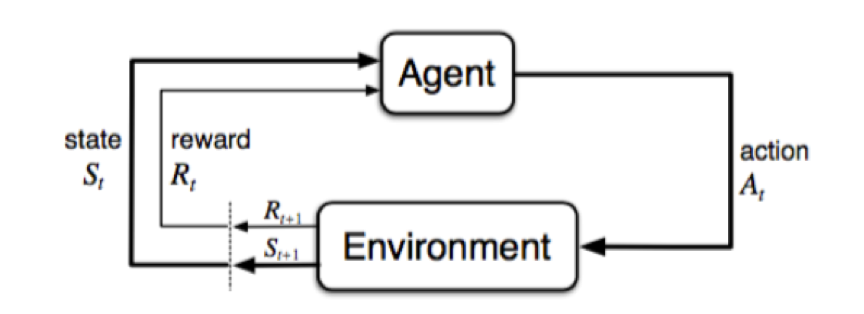
\includegraphics[width=\columnwidth]{Figures/MDP}
\decoRule
\caption[Markov Decision Process]{Markov Decision Process (\cite{sutton1998introduction})}
\label{fig:MDP}
\end{figure}

\paragraph{}
Taken the chess example again, each time the player receive a state $s$, in this case, the chess board situation. The player could choose an action that is viable under current state $s$. Assume the player chooses action $a$, the environment, in this case, the chess rule, will transit the state $s$ into a new state $s^{\prime}$, also giving the player a reward $r$. The reward may be small when you eat a pawn while it may be big when you win the game. 
\paragraph{}
One core property of Markov decision process is that the transition obeys Markov property. Markov property means the probability that the process moves into its new state $s^{\prime}$ is influenced only by the chosen action $a$ and current state $s$. Specifically, it is given by the state transition function $T(s,a,s^{\prime})$. Given $s$ and $a$, it is conditionally independent of all previous states and actions. 
\paragraph{}
Markov property makes it possible to analyze the action selection by only looking at the current state because current state contains all information the decision maker need to know, otherwise the Markov property is unsatisfied. It is obvious that the chess example has Markov property since the information on board, $s$, is sufficient for the player to make its action and transit to a new state (ignore the influence to board caused by opponents). 
% TODO MDP consist of S,A,T,R,\gamma
\paragraph{}
This thesis will focus on Markov decision process only because of the simplicity of Markov property. 
%----------------------------------------------------------------------------------------



%----------------------------------------------------------------------------------------
\section{Thesis Structure}
\paragraph{}
Sequential decision making are so essential that our life may fall apart without such ability. Hence, there has been much work inspecting the process of sequential decision making, especially Markov decision process. In this thesis, I will also try to design an experiment to explore several possible decision methods under Markov devision process. 
\paragraph{}
We have given introduction of the sequential decision making problem and its formalized framework Markov Decision Process in Chapter \ref{Chapter 1}. We will introduce several existing work in this topic in Chapter \ref{Chapter 2}. After that, we will present our experiment in Chapter \ref{Chapter 3}. Chapter \ref{Chapter 4} will be basic statistical analyses and in Chapter \ref{Chapter 5} we will put forward several models that are theoretically possible in our task and compare them with classic ones. Finally, we will discuss and conclude what we have discovered with some future research directions. 
%----------------------------------------------------------------------------------------
% Chapter 2

\chapter{Chapter 2: Background Theory} % Main chapter title

\label{Chapter 2} % For referencing the chapter elsewhere, use \ref{Chapter2} 

%----------------------------------------------------------------------------------------
\section{Reinforcement Learning}
\paragraph{}
From Thorndike's Law of Effect, Pavlov's classical conditioning and Skinner's operant conditioning, people are trying to connect the consequence to the behavior (\cite{thorndike1927law}). Reinforcement learning (RL) is initially a psychology term to explain the phenomenon that people will increase the probability of doing something after positive stimulation such as reward and will decrease the probability after negative stimulation such as electric shock (similar to operant conditioning) (\cite{dayan2002reward}). In the 1980s, reinforcement learning is introduced to machine learning area, concerned with how software agents ought to take actions in an environment so as to maximize some notion of cumulative reward. 
\paragraph{}
It is widely accepted that reinforcement learning is the proper solution to Markov decision process. Most recently, reinforcement learning in computer science has been experiencing a boost due to its great success on several tasks such as Go and Atari games (\cite{mnih2015human}). 
\paragraph{}
At the same time, reinforcement learning in psychology and neuroscience have made great advancement. \citet{hollerman1998dopamine} discovered that dopamine neurons in midbrain have the corresponding activity with reward prediction error, which is the core element of Model-Free learning. This pattern is also frequently reported in later work (\cite{bayer2005midbrain}; \cite{waelti2001dopamine}). Human fMRI results also prove that stratum does have stronger activity when reward prediction error is positive (\cite{garrison2013prediction}; \cite{kishida2016subsecond}). 
\paragraph{}
Therefore, reinforcement learning has been proven effective both empirically and theoretically. What's more, it is viable in human brain via midbrain dopamine system. Taken all pieces together, reinforcement learning seems to become the most convincing theory in modeling sequential decision making. Thus, we will introduce several reinforcement learning algorithms in this section. We will also build our models on top of classic reinforcement learning algorithms in Chapter \ref{Chapter 5}. 
%----------------------------------------------------------------------------------------


%----------------------------------------------------------------------------------------
\section{Model-Free Algorithm Family}
\paragraph{}
Model-Free means the participant or agent does not build a model for the environment explicitly but to maintain a value estimation for each state-action pair. 

\paragraph{}
The Model-Free algorithm family mainly includes SARSA and Q-learning. To understand Model-Free algorithm, first we need to define \enquote{Q value} as in Equation \ref{eqn:Q definition}. The Q value represents how much value can I get in the long run after taking action $a$ in state $s$. Note that the value considers long run outcome rather than immediate outcome. According to this definition, if we could get the true Q value, we should just always choose the action with maximum Q value to gain the best performance. So, how do we calculate Q value?

\begin{equation}
\begin{aligned}
Q(s,a)=\sum_{t=0}^\infty{\gamma^tR(s_t)}
\end{aligned}
\label{eqn:Q definition}
\end{equation}

\paragraph{}
There are two classic methods to estimate Q value in the model-free manner: SARSA and Q-learning (\cite{daw2014algorithmic}). They are both motivated by reward prediction error (RPE). Reward prediction error is defined as the difference between the expected value and the real encountered value. If a participant receives a positive RPE, he will know that his prediction is underestimated and should be increased. If a participant receives a negative RPE, he will inversely decrease his value estimation. SARSA and Q-learning formulation are shown in Equation \ref{eqn:SARSA0} and \ref{eqn:Q-Learning0}. 
\paragraph{}
The difference between SARSA and Q-learning is that when calculating reward prediction error (RPE), SARSA uses the true action chosen by participants in the next timestep, while Q-learning uses the action with maximum Q value on the next state.

\begin{equation}
\begin{aligned}
&\delta_{RPE}=r(s^{\prime})+\gamma Q_{SARSA}(s^{\prime}, a^{\prime})-Q_{SARSA}(s,a) \\
&Q_{SARSA}(s,a)=Q_{SARSA}(s,a)+\alpha \delta_{RPE} \\
\end{aligned}
\label{eqn:SARSA0}
\end{equation}

\begin{equation}
\begin{aligned}
&\delta_{RPE}=r(s^{\prime})+\gamma \max_{a^{\prime} \in a(s)}{Q_{Q}(s^{\prime}, a^{\prime})}- Q_{Q}(s,a) \\
&Q_Q(s,a)=Q_Q(s,a)+\alpha \delta_{RPE} \\
\end{aligned}
\label{eqn:Q-Learning0}
\end{equation}

\paragraph{}
Model-Free algorithms requires little computation but needs fair amount of storage because it need to store all the state-action pair values. However, Model-Free algorithms suffer from environment change because they could only re-learn the Q value when either transition $T$ or reward $R$ has been changed. 

%----------------------------------------------------------------------------------------



%----------------------------------------------------------------------------------------
\section{Model-Based Algorithm Family}
\paragraph{}
Unlike Model-Free algorithms, Model-Based algorithm maintain an explicit representation of the environment, i.e. the transition matrix $T$ and reward function $R$. The learning method of $T$ and $R$ will be explained in Chapter \ref{Chapter 5}. Here we will first explain several methods to calculate value estimation using estimated $T$ and $R$. 
\paragraph{}
The first intuitive method is to use the definition of value function to calculate v by regarding the estimated $T$ and $R$ as true $T$ and $R$. 

\begin{equation}
\begin{aligned}
Q(s,a)=\hat{r} + \gamma \hat{T}\hat{R} + \gamma^2\hat{T}^2\hat{R} + ...
\end{aligned}
\label{eqn:Enumeration}
\end{equation}

\paragraph{}
The second way is to use bellman equation (\cite{sutton1998introduction}) $Q = R+ \gamma TQ$. Specifically, we could build an iteration algorithm to do value iteration by Equation \ref{eqn:Consistency}, in which $Q_{t}$ represents t-th iteration Q. 

\begin{equation}
\begin{aligned}
Q_{t+1}=\hat{R}+\gamma \hat{T}Q_{t}
\end{aligned}
\label{eqn:Consistency}
\end{equation}

\paragraph{}
In order to decrease the computation complexity, we could also do Monte-Carlo sampling for transition matrix $T$. 

\paragraph{}
Model-based method requires a lot of computation but are able to adjust to environment changes. For instance, when reward function changes, as long as the participant has learned the transition structure of the environment, he will still be able to obtain the reward. 

%----------------------------------------------------------------------------------------



%----------------------------------------------------------------------------------------
\section{Other Algorithms}
\paragraph{}
There has been much work about Model-Free and Model-Based combination method. \citet{daw2005uncertainty} and \citet{doya2002multiple} suggests that Model-Free and Model-Based value estimation may be combined in proportion to their certainty about their value estimation. \citet{glascher2010states} introduces a hybrid model whose hybrid weight is a exponential function. \citet{daw2011model} claims that Model-Based and Model-Free work simultaneously in our decision making. 

\paragraph{}
Except MF model, MB model and their combination, their still exists many other computational models. \citet{gershman2017reinforcement} argues that reinforcement learning is tightly bound to episodic memory and use a kernel function to make new predictions. \citet{botvinick2015reinforcement} and \citet{botvinick2012hierarchical} bring forward a hierarchical model of reinforcement learning. The main idea of hierarchical RL is to combine some action sequence as a new action for participants to choose. 
%----------------------------------------------------------------------------------------







 
% Chapter 3

\chapter{Chapter 3: Experiment} % Main chapter title

\label{Chapter 3} % For referencing the chapter elsewhere, use \ref{Chapter3} 

%----------------------------------------------------------------------------------------
\section{Experiment Intuition}
\label{sec:Experiment Intuition and Environment}
\paragraph{}
Existing experiments are generally simple both in state space and temporal structure, such as \citet{glascher2010states}, \citet{daw2011model}. They only examine the RL process in a two-stage decision making task. There is no evidence which RL algorithm will work when the problem becomes complicated. 

\paragraph{}
Besides, it seems that less is known about multi-task decision making. Previous work mostly use one reward function to see the learning process. But we do not know whether multiple-task simultaneous learning will cause tasks to assist or interfere with each other. 

\paragraph{}
Finally, the orders of tasks may further change the assistance or interference. 

\paragraph{}
With these questions, we defined our own experiment environment. 

\section{Experiment Environment}
\label{sec:Experiment Environment}
\subsection{Environment Structure}
\label{sec:Experiment Environment}
\paragraph{}
We create an abstract "labyrinth" environment for human to play. The labyrinth structure is displayed in Fig. \ref{fig:Environment Structure}. Each circle and the corresponding character represents a "state" participants may be in. The lines between states represents action's primary resulting states (we will explain the word "primary" in Section \ref{sec:Experiment Details}. Right now, you could just regard where the line points is its resulting state). It is obvious that the labyrinth consists of 6 states and each state has 3 actions, which point to 3 different resulting states. The goal for participants is to move from one state to another. For example, the participants may be asked to migrate from state \emph{A} to state \emph{B}. In this situation, the optimal solution is firstly move from \emph{A} to \emph{E}, and then go straight to \emph{B}. As a result, he successfully transmit himself from \emph{A} to \emph{B} in two steps. It is worth noting that participants know nothing about the structure of this environment before acting. Therefore, they could only know the structure by trying and learning. 

\begin{figure}[ht]
\centering
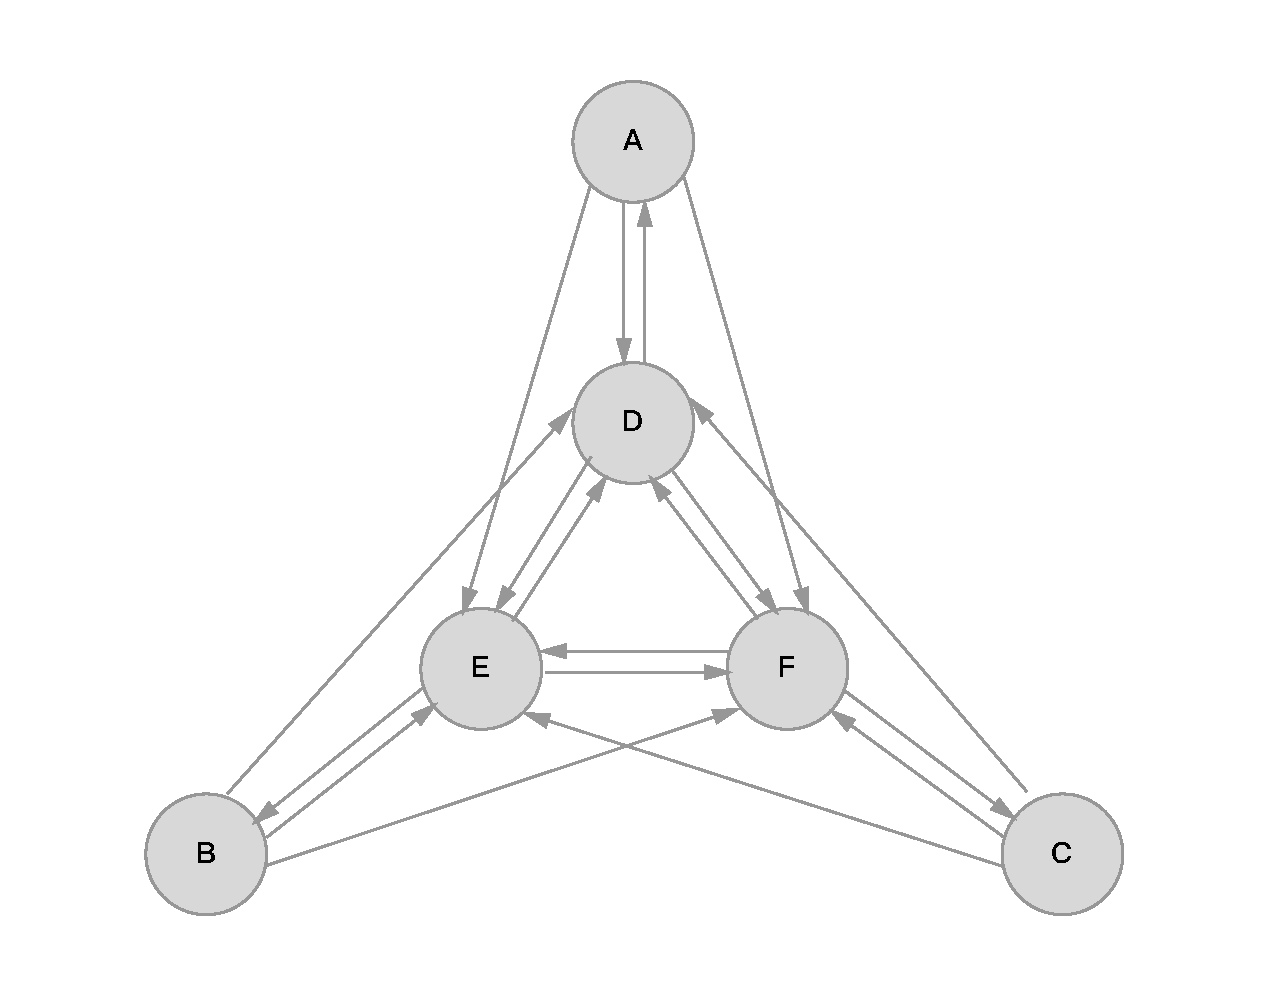
\includegraphics[width=\columnwidth]{Figures/environment_structure}
\decoRule
\caption[Environment Structure]{Environment Structure: circle indicates states (including \emph{A}, \emph{B}, \emph{C}, \emph{D}, \emph{E}, \emph{F}), line indicates action's primary consequence. }
\label{fig:Environment Structure}
\end{figure}

\paragraph{}
In this task, each states is represented by a fractal image, as shown in Fig. \ref{fig:fractal}. We chose 6 dissimilar fractal images to represent 6 different states. 

\begin{figure}[ht]
\centering
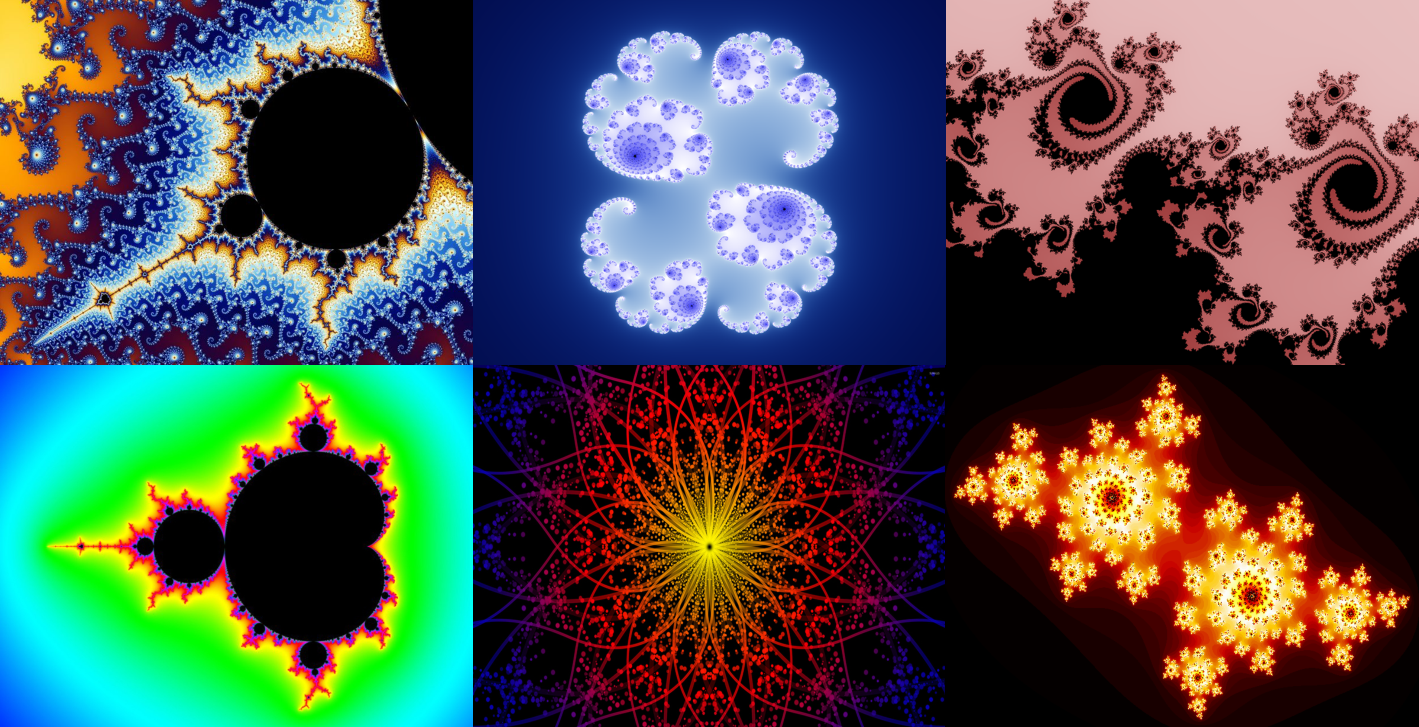
\includegraphics[width=\columnwidth]{Figures/fractal}
\decoRule
\caption{States Fractal Image}
\label{fig:fractal}
\end{figure}

\subsection{Trial Procedure}
\label{sec:Trial Procedure}
\paragraph{}
The Trial Procedure is demonstrated in Fig. \ref{fig:Experiment Procedure}. 
\paragraph{}
In the beginning of each trial, a fixation is displayed at the screen center for 1 second. After that, the trial start state and goal state are shown (start state at center, end state on the right) for 1.5 seconds. This is called preparation phase. Then, the free choice phase begins. 
\paragraph{}
At each timestep of free-choice phase, the state which the participant is now in is displayed in the center, being surrounded by three arrows indicating three kinds of actions. The goal state is always displayed on the right as in the preparation phase. Besides, there is a reward indication below the state, showing how much tokens participant could get if he reaches the end state after the next action. After the participant has made his decision and pressed one of three buttons, the center image will transit to the outcome state image with a fade-in fade-out fashion (previous image's $\alpha$ decreased gradually and new image's $\alpha$ increased gradually). In the meantime, reward indication will decrease by 1 (initially 20). But if the reward has been 1, it will not decrease but remain 1. There is no maximum reaction time, which means the screen will remain unchanged unless the participant press a button. When the transition ends, a new timestep begins. This is repeated until the state that participant is in reaches the end state. 
\paragraph{}
If participants have reached the end state, the trial enters feedback phase, in which total steps the participant takes to move to the end state and tokens earned are shown for 3 seconds. After feedback phase, a new trial begins with fixation. 

\begin{figure}[ht]
\centering
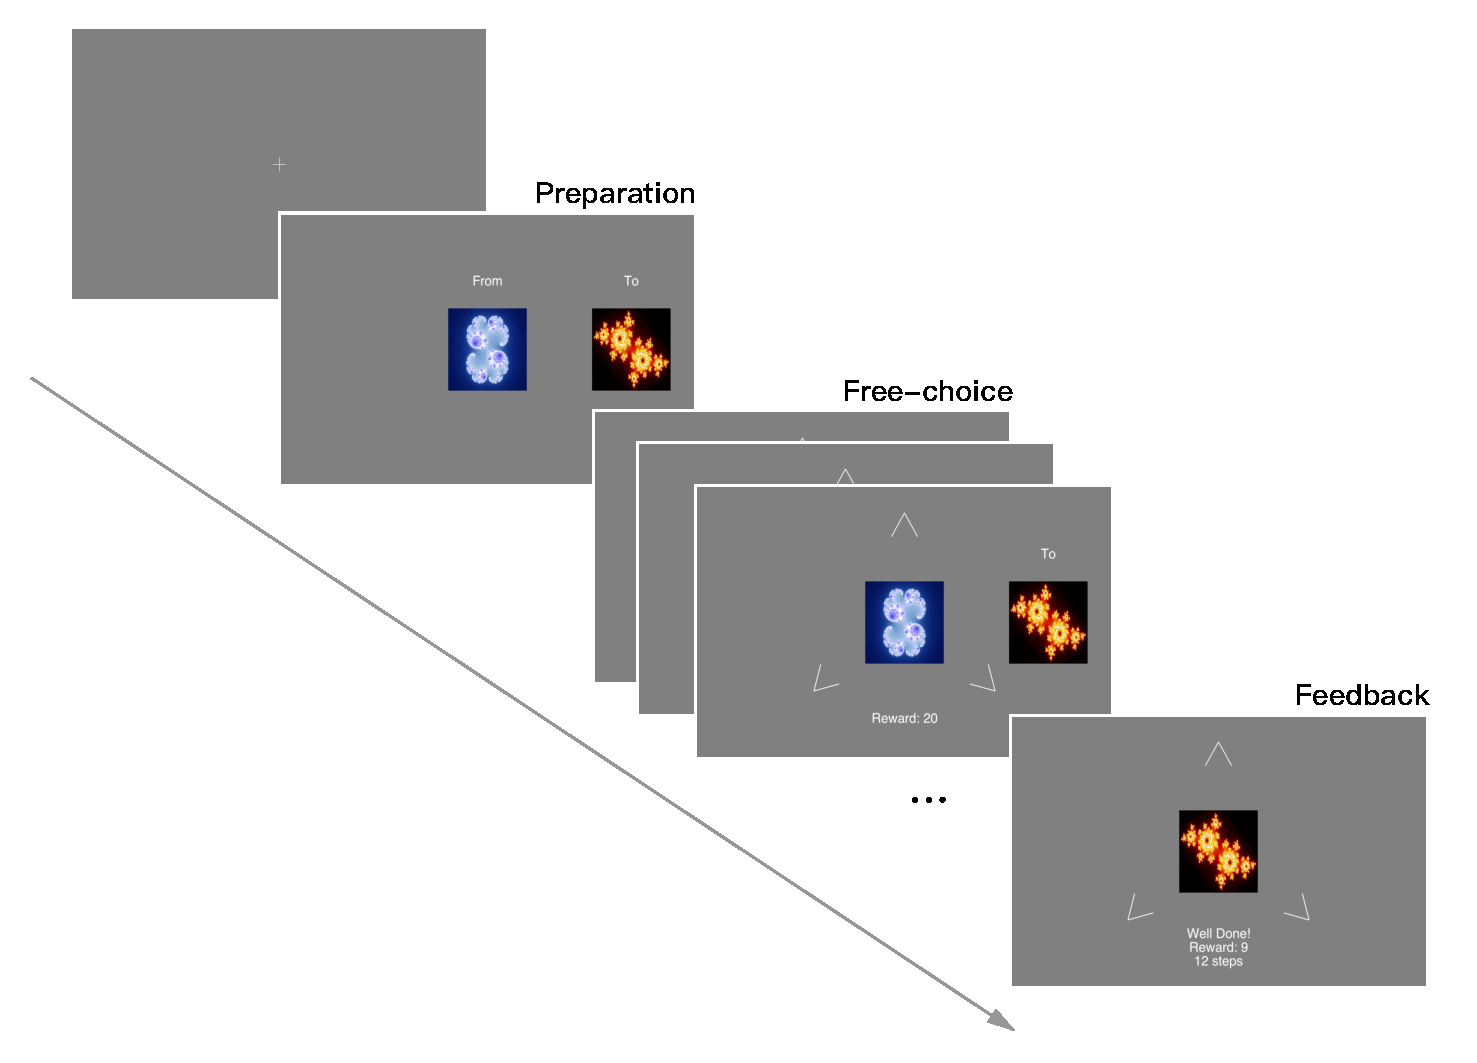
\includegraphics[width=\columnwidth]{Figures/experiment_procedure}
\decoRule
\caption{Experiment Procedure}
\label{fig:Experiment Procedure}
\end{figure}
%----------------------------------------------------------------------------------------


%----------------------------------------------------------------------------------------
\section{Experiment Design}
\label{sec:Experiment Design}
\paragraph{}
For every participant, there are totally 144 trials. each trial follows the procedure described in Section \ref{sec:Trial Procedure}. Till now, we haven't described how the start state and end state are chosen for each trial, and that's the key point of experiment design. 
\paragraph{}
The experiment is a between-subject design. The between-subject independent variable is the order of tasks and have two levels: randomized and block. Participants with odd participant id are assigned to block condition while participants with even participant id are assigned to randomized condition. For all conditions, whether randomized or block, the experiment consists of three kinds of start-end pairs: \emph{A} to \emph{B}, \emph{B} to \emph{C} and \emph{C} to \emph{A}. In short, the \enquote{inner} state \emph{D}, \emph{E}, \emph{F} will not be used as start or end state. The reason why we choose such tasks is that every task has an optimal solution of two steps. Just as the example shown in \ref{sec:Experiment Environment}, if the participant is asked to transit from \emph{A} to \emph{B}, he should take the path of \emph{A} -> \emph{E} -> \emph{B}, which takes two steps. You may also be wondering why we do not choose the opposite direction tasks, such as \emph{B} to \emph{A} as well. It is because we want to examine the possibility of knowledge transfer from previous tasks to newly occurred goals. For example, after learning how to move from \emph{A} to \emph{B} and from \emph{B} to \emph{C}, the participants are asked to do the task of \emph{C} to \emph{A}. In this manner, we want to test whether participants could transfer any knowledge from previous tasks, for instance, the structure of of environment, to the new tasks. That is exactly the difference between model-free and model-based algorithms. The overall trial number for each participant is 144. We divide 144 trials averagely into three tasks (\emph{A} to \emph{B}, \emph{B} to \emph{C} and \emph{C} to \emph{A}), making each one 44 trials. 
\paragraph{}
The experiment has 4 blocks, each of which contains 36 trials. 
For randomized condition, participants' tasks are assigned pseudo-randomly. For block condition, participants will only learn \emph{A} to \emph{B} in the first block, and then learn \emph{B} to \emph{C} in the second block, learn \emph{C} to \emph{A} in the third block. The final block of block condition consists of 12 trials for each task and the order is randomly assigned. In short, under randomized condition participants will learn all three tasks simultaneously while under block condition participants will learn the task one by one and finally test in the last block. 
%----------------------------------------------------------------------------------------


%----------------------------------------------------------------------------------------
\section{Experiment Details}
\label{sec:Experiment Details}
\paragraph{}
Now it is clear how the trial tasks are assigned and how a single trial proceeds. We still have several experiment details to explain. 
\paragraph{}
For the mapping from abstract state characters (such as \emph{A}) to fractal images, each participants received a randomly assigned mapping. In this case, the effect that specific images may cause can be balanced. 
\paragraph{}
For the mapping from state's action to \enquote{primary} consequence, it is also randomly assigned for each participant to avoid the possibility that specific optimal solution is preferred and relatively easy to learn for participants. 
\paragraph{}
The action's \enquote{primary} consequence mentioned in Section \ref{sec:Experiment Environment} means that in fact, action's consequence is stochastic in this environment. For a specific action of a state, it will have $0.7$ probability to transit to the primary consequence. However, it still have $0.2$ and $0.1$ probability to transit to other action's primary consequence of the same state. For example, the state \emph{A}'s first action's primary consequence is \emph{E}, while second action's primary consequence is \emph{D} and third action's primary consequence is \emph{F}. In this case, when participants chose the first action in state \emph{A}, it will transit to \emph{E} with probability $0.7$ and will transit to \emph{D} or \emph{F} with probability $0.2$ or $0.1$ (the one with $0.2$ probability is called \enquote{secondary} consequence, which is determined together with \enquote{primary} consequence when the environment is created). Thus, the action's consequence is stochastic actually. The reason why we add stochasticity here is to increase difficulty of the task, making it hard for participants to find the structure of our environment. As we mentioned in Section \ref{Chapter 1}, the existing work is mainly focused on laboratory toy problems, rather than real-world complex decision making. Though the complexity is still not comparable to real-world situations, it has been much more complex than previous tasks. 
\paragraph{}
The data our experiment records is the whole decision process, including every timestep's data of every trial. Each timestep data consists of current state, action chosen by participants, transition resulting state and reaction time. We will show how we analyze data in the following chapters. 
\paragraph{}
As for the reward, all the rewards participants collected in the experiment are tokens. The participant fee is calculated by $fee = 30 + tokens / 100$. An average participant may gain a fee of approximately 50 CNY. 
\paragraph{}
The data is collected on 36 Peking University students. They all have normal vision or corrected normal vision, including color vision. All participants had given informed consent before the experiment. 
%----------------------------------------------------------------------------------------





% Chapter 4

\chapter{Chapter 4: Statistical Analysis} % Main chapter title

\label{Chapter 4} % For referencing the chapter elsewhere, use \ref{Chapter4} 

\paragraph{}
In this chapter, we will firstly calculate several metrics according to the participants' data and show the descriptive statistics. After that we will use statistical test to prove that learning does occur in both randomized and block conditions. 

%----------------------------------------------------------------------------------------
\section{Metrics Definition}
\label{sec:Metrics Definition}
\paragraph{}
As we mentioned in Section \ref{sec:Experiment Details}, we record each timestep's data of each trial, including current state, action chosen by participants, transition resulting state and reaction time. It is hard to directly analyze sequential data as in this experiment, thus we calculate several metrics for each trial, and analyze them on the trial dimension. 
\subsection{Steps}
\label{sec:Steps}
\paragraph{}
Number of steps is the most straightforward metric to measure a trial. It is obvious that the less steps participants takes, the better his policy is. This metric is named \enquote{step}. Participants' step data is shown in Fig. \ref{fig:Step Participants}. 

\begin{figure}[ht]
\centering
\subfigure[Randomized Condition]{
\begin{minipage}[t]{0.48\textwidth}
\centering
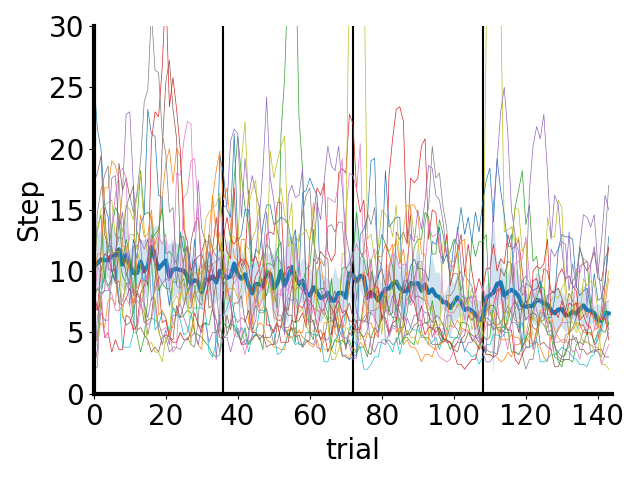
\includegraphics[width=\textwidth]{Figures/steps_randomized_participants}
\end{minipage}
}
\subfigure[Block Condition]{
\begin{minipage}[t]{0.48\textwidth}
\centering
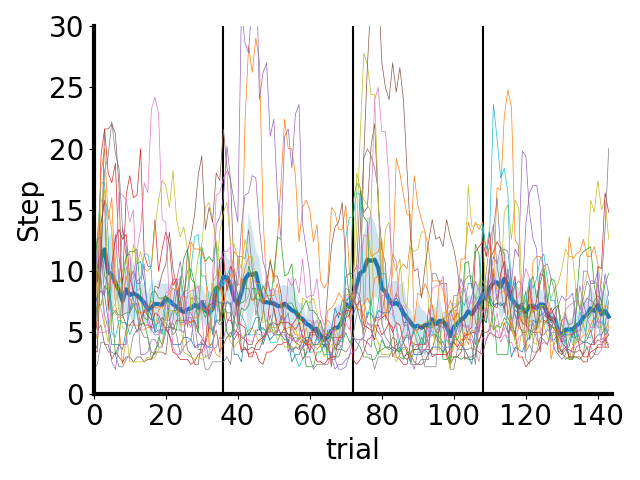
\includegraphics[width=\textwidth]{Figures/steps_block_participants}
\end{minipage}
}
\decoRule
\caption[Step data of participants]{Step data of participants in (a) randomized condition (b) block condition. The thick blue line is the mean of all participants (blue shadow indicating standard error), while the thin colorful lines are data of each participant. Vertical lines on 36, 72, 108 indicate block separation. }
\label{fig:Step Participants}
\end{figure}



\subsection{Reaction Time and Normalized Reaction Time}
\label{sec:Reaction Time and Normalized Reaction Time}
\paragraph{}
The reaction time of each timestep is recorded in data. Hence, we could sum all the reaction time of all the timesteps in one trial to represent participants' overall decision making time in a single trial. This metric is named \enquote{Reaction Time}. Participant's reaction time data is shown in Fig. \ref{fig:Reaction Time Participants}. 

\begin{figure}[ht]
\centering
\subfigure[Randomized Condition]{
\begin{minipage}[t]{0.48\textwidth}
\centering
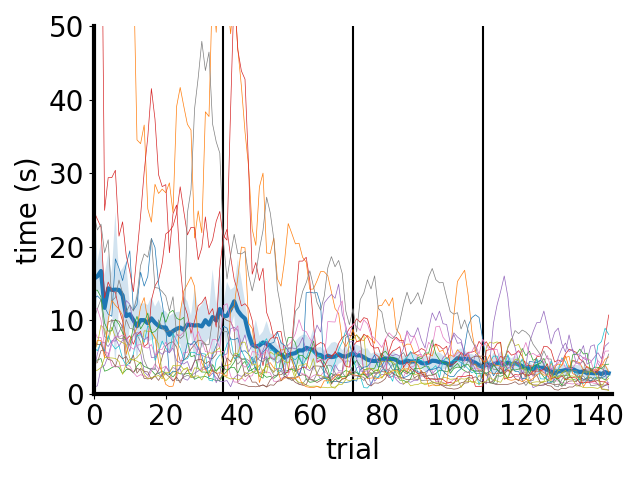
\includegraphics[width=\textwidth]{Figures/time_randomized_participants}
\end{minipage}
}
\subfigure[Block Condition]{
\begin{minipage}[t]{0.48\textwidth}
\centering
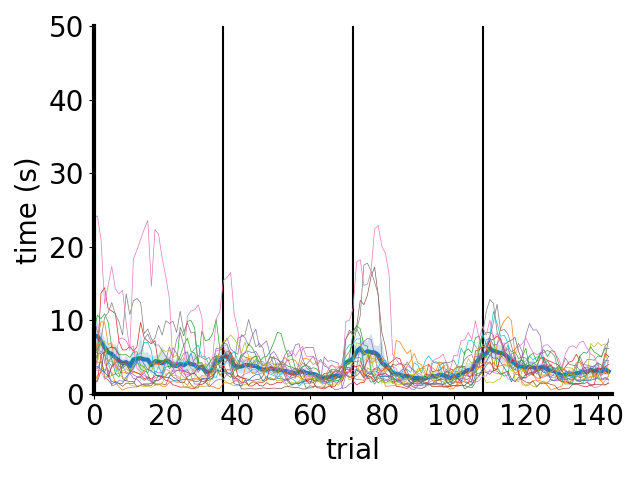
\includegraphics[width=\textwidth]{Figures/time_block_participants}
\end{minipage}
}
\decoRule
\caption[Reaction time data of participants]{Reaction time data of participants in (a) randomized condition (b) block condition. The thick blue line is the mean of all participants (blue shadow indicating standard error), while the thin colorful lines are data of each participant. Vertical lines on 36, 72, 108 indicate block separation. }
\label{fig:Reaction Time Participants}
\end{figure}

\paragraph{}
It is obvious that the \enquote{Reaction Time} metrics is strongly influenced by \enquote{Step} because of the sum operation. Thus, we create a new metric named \enquote{Normalized Reaction Time} to decrease the influence of \enquote{Step} by dividing \enquote{Reaction Time} with \enquote{Steps}. Fig \ref{fig:Normalized Reaction Time Participants} shows \enquote{Normalized Reaction Time} in participants. 

\begin{figure}[ht]
\centering
\subfigure[Randomized Condition]{
\begin{minipage}[t]{0.48\textwidth}
\centering
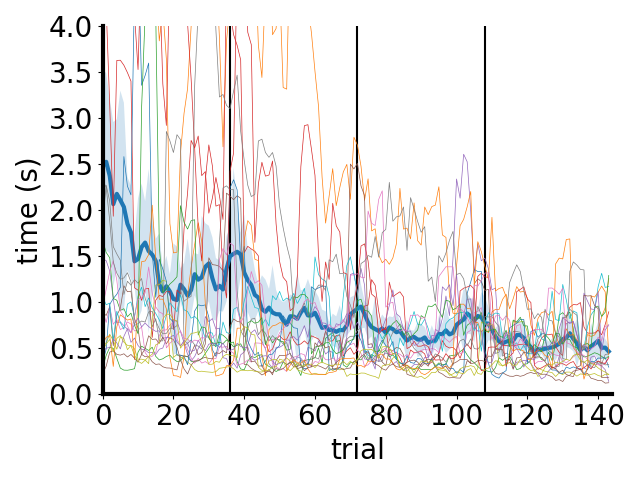
\includegraphics[width=\textwidth]{Figures/normalized_time_randomized_participants}
\end{minipage}
}
\subfigure[Block Condition]{
\begin{minipage}[t]{0.48\textwidth}
\centering
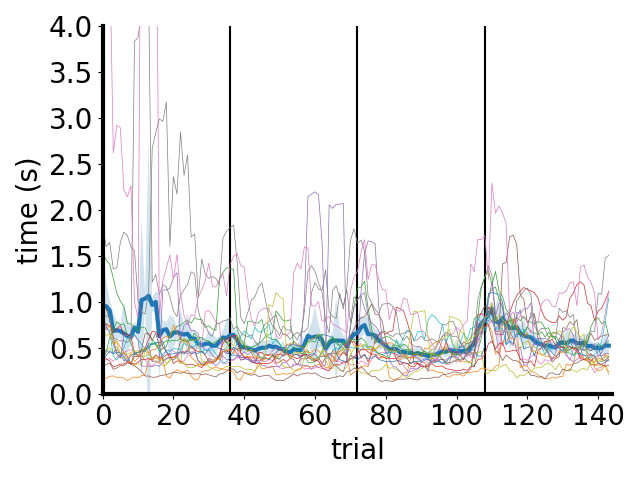
\includegraphics[width=\textwidth]{Figures/normalized_time_block_participants}
\end{minipage}
}
\decoRule
\caption[Normalized Reaction time data of participants]{Normalized Reaction time data of participants in (a) randomized condition (b) block condition. The thick blue line is the mean of all participants (blue shadow indicating standard error), while the thin colorful lines are data of each participant. Vertical lines on 36, 72, 108 indicate block separation. }
\label{fig:Normalized Reaction Time Participants}
\end{figure}


\subsection{Optimal Percentage}
\label{sec:Optimal Percentage}
\paragraph{}
All three metrics mentioned above are all straightforward from raw data. But we are most interested in how participants learn to play this task well. For this purpose, we defined several Optimal-related metrics to indicate how participants learn this task step by step. 
\paragraph{}
First we need to define \enquote{optimal}. At each state the participant is in, there exists an optimal action choose. For instance, if the goal is \emph{B}, the optimal action in \emph{A}, \emph{D}, \emph{F}, \emph{C} will all be the one whose primary consequence is \emph{E}, while the optimal action in \emph{E} is the one whose primary consequence is \emph{B}. This action is called \enquote{optimal action}. 
\paragraph{}
Thus, we could calculate whether at each timestep the participant choose the optimal action. Then we are able to calculate the optimal action percentage in each trial, making it a trial metric. This metric is called \enquote{Optimal Percentage} and its trend with trial is shown in Fig. \ref{fig:Optimal Percentage Participants}. 

% TODO increase figure axis font and thickness of axis
\begin{figure}[ht]
\centering
\subfigure[Randomized Condition]{
\begin{minipage}[t]{0.48\textwidth}
\centering
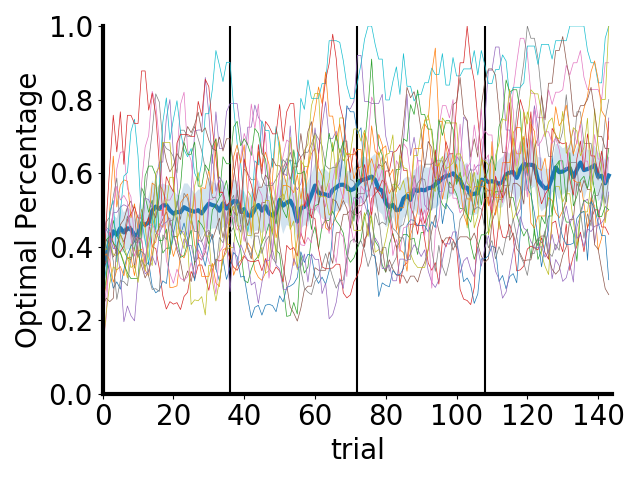
\includegraphics[width=\textwidth]{Figures/optimal_randomized_participants}
\end{minipage}
}
\subfigure[Block Condition]{
\begin{minipage}[t]{0.48\textwidth}
\centering
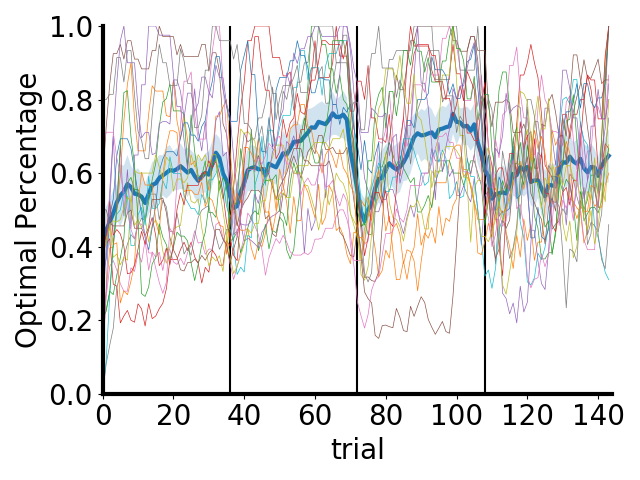
\includegraphics[width=\textwidth]{Figures/optimal_block_participants}
\end{minipage}
}
\decoRule
\caption[Optimal Percentage data of participants]{Optimal Percentage data of participants in (a) randomized condition (b) block condition. The thick blue line is the mean of all participants (blue shadow indicating standard error), while the thin colorful lines are data of each participant. Vertical lines on 36, 72, 108 indicate block separation. }
\label{fig:Optimal Percentage Participants}
\end{figure}

\paragraph{}
In order to examine participants' learning more precisely, we divide the state into three categories: \enquote{inner}, \enquote{outer}, \enquote{last}. For each trial with a end state \emph{X}, the \enquote{last} category includes only the one that can directly move to end state \emph{X}. For instance, if the end state is \emph{B}, then the \enquote{last} category includes only \emph{E} (the environment structure can be found in Fig. \ref{fig:Environment Structure}). The \enquote{inner} category includes two of three inner states \emph{D}, \emph{E}, \emph{F} except the one included in the \enquote{last} category, which in this example means the \enquote{inner} category includes \emph{D} and \emph{F}. Finally the \enquote{outer} category includes two of three outer states \emph{A}, \emph{B}, \emph{C} except the end state, which in this instance means \emph{A} and \emph{C}. Optimal Percentage in three state categories are named as \enquote{Inner Optimal Percentage}, \enquote{Outer Optimal Percentage} and \enquote{Last Optimal Percentage}. Participants' data on these three metrics are shown in Fig. \ref{fig:Inner Optimal Percentage Participants}, Fig. \ref{fig:Outer Optimal Percentage Participants} and Fig. \ref{fig:Last Optimal Percentage Participants}.

\begin{figure}[ht]
\centering
\subfigure[Randomized Condition]{
\begin{minipage}[t]{0.48\textwidth}
\centering
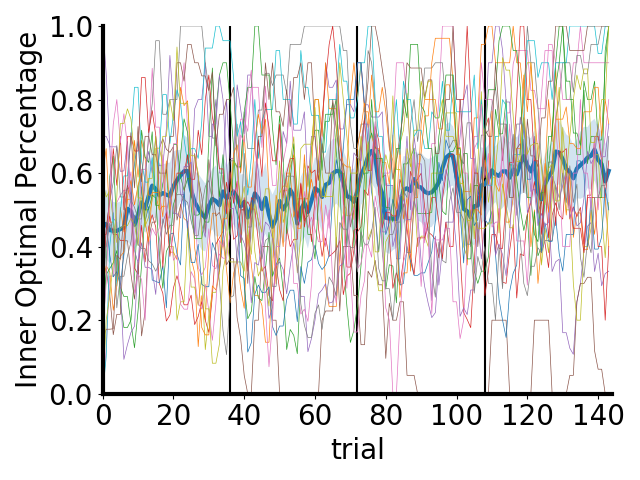
\includegraphics[width=\textwidth]{Figures/optimal_inner_randomized_participants}
\end{minipage}
}
\subfigure[Block Condition]{
\begin{minipage}[t]{0.48\textwidth}
\centering
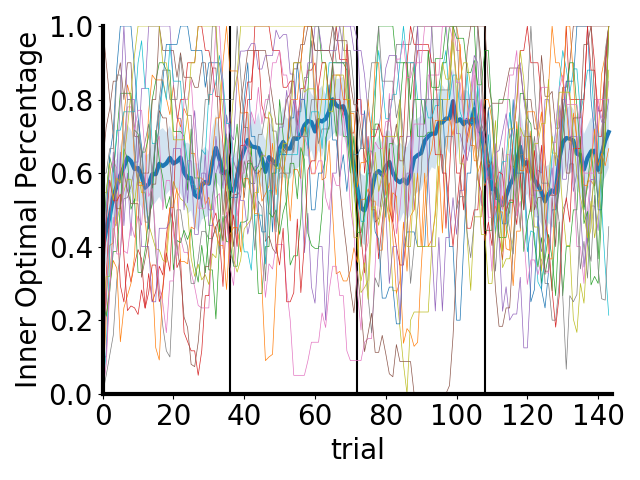
\includegraphics[width=\textwidth]{Figures/optimal_inner_block_participants}
\end{minipage}
}
\decoRule
\caption[Inner Optimal Percentage data of participants]{Inner Optimal Percentage data of participants in (a) randomized condition (b) block condition. The thick blue line is the mean of all participants (blue shadow indicating standard error), while the thin colorful lines are data of each participant. Vertical lines on 36, 72, 108 indicate block separation. }
\label{fig:Inner Optimal Percentage Participants}
\end{figure}

\begin{figure}[ht]
\centering
\subfigure[Randomized Condition]{
\begin{minipage}[t]{0.48\textwidth}
\centering
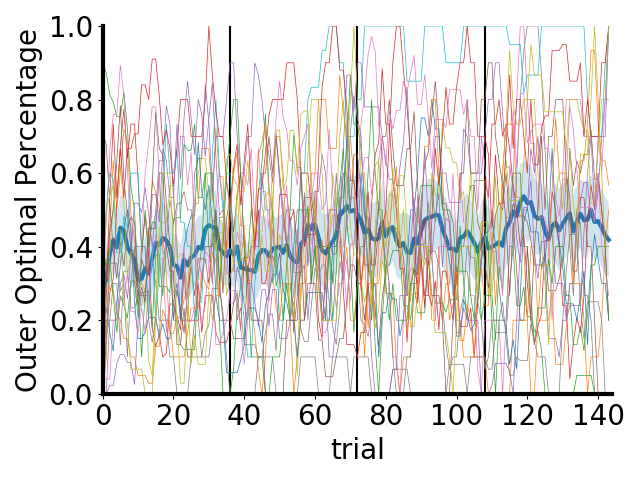
\includegraphics[width=\textwidth]{Figures/optimal_outer_randomized_participants}
\end{minipage}
}
\subfigure[Block Condition]{
\begin{minipage}[t]{0.48\textwidth}
\centering
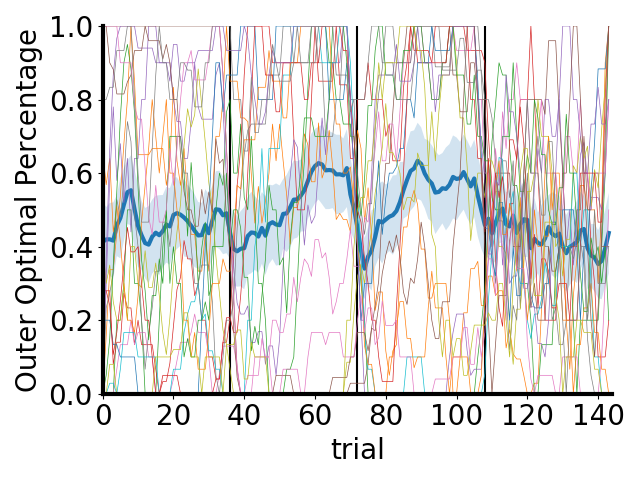
\includegraphics[width=\textwidth]{Figures/optimal_outer_block_participants}
\end{minipage}
}
\decoRule
\caption[Outer Optimal Percentage data of participants]{Outer Optimal Percentage data of participants in (a) randomized condition (b) block condition. The thick blue line is the mean of all participants (blue shadow indicating standard error), while the thin colorful lines are data of each participant. Vertical lines on 36, 72, 108 indicate block separation. }
\label{fig:Outer Optimal Percentage Participants}
\end{figure}

\begin{figure}[ht]
\centering
\subfigure[Randomized Condition]{
\begin{minipage}[t]{0.48\textwidth}
\centering
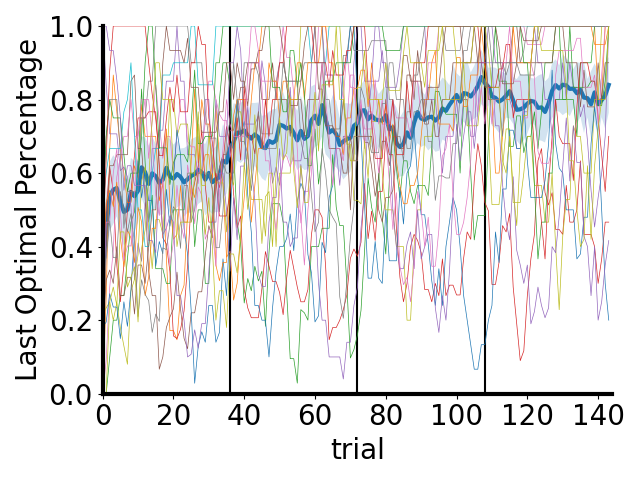
\includegraphics[width=\textwidth]{Figures/optimal_last_randomized_participants}
\end{minipage}
}
\subfigure[Block Condition]{
\begin{minipage}[t]{0.48\textwidth}
\centering
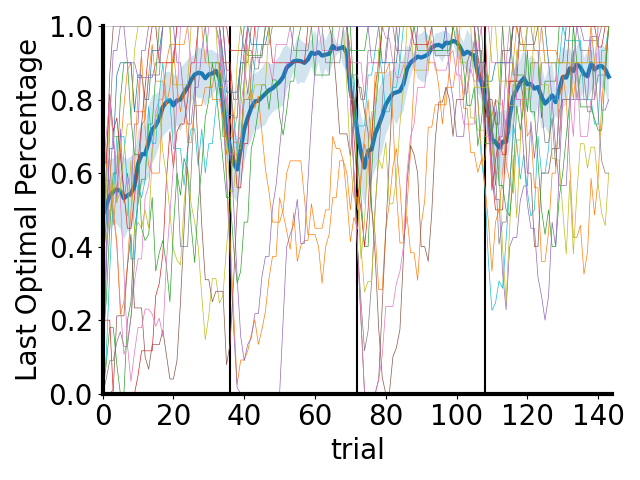
\includegraphics[width=\textwidth]{Figures/optimal_last_block_participants}
\end{minipage}
}
\decoRule
\caption[Last Optimal Percentage data of participants]{Last Optimal Percentage data of participants in (a) randomized condition (b) block condition. The thick blue line is the mean of all participants (blue shadow indicating standard error), while the thin colorful lines are data of each participant. Vertical lines on 36, 72, 108 indicate block separation. }
\label{fig:Last Optimal Percentage Participants}
\end{figure}

\paragraph{}
The advantage of \enquote{Optimal Percentage} over \enquote{Step} is that it will not be influenced by the stochasticity of the transition (action stochastic consequence), while \enquote{Step} is strongly influenced by the transition randomness even if all the actions chosen by participants are optimal. What's more, \enquote{Optimal Percentage} is a variable between 0 and 1 while \enquote{Step} does not have an upper bound, making \enquote{Optimal Percentage} metric having better statistical properties. 
\paragraph{}
The reason why we further divide \enquote{Optimal Percentage} into three categories is that we assume participants may take different learning process for each different states. For example, it is obvious that \enquote{last} category is the most simple to learn. In the meantime, it seems that participants learn \enquote{inner} category much better than \enquote{outer} category. In this way, we may divide participants' learning in three different kinds of states. 
\paragraph{}
All 7 metrics are summarized in Table \ref{table:All Metrics}, and the last column indicates whether or not it can be reflected in model simulation in Section \ref{sec:Model Simulation}. 

\begin{table}
\caption{All Metrics in Data Analysis}
\label{table:All Metrics}
\centering
\begin{tabular}{l c c}
\toprule
\tabhead{Metric Name}& \tabhead{Bound} & \tabhead{Simulation Reflected} \\
\midrule
Step & [2, Inf) & ${\surd}$ \\
Reaction Time & (0, Inf) & ${\times}$ \\
Normalized Reaction Time & (0, Inf) & ${\times}$ \\
Optimal Percentage & [0, 1] & ${\surd}$ \\
Inner Optimal Percentage & [0, 1] & ${\surd}$ \\
Outer Optimal Percentage & [0, 1] & ${\surd}$ \\
Last Optimal Percentage & [0, 1] & ${\surd}$ \\
\bottomrule\\
\end{tabular}
\end{table}
%----------------------------------------------------------------------------------------



%----------------------------------------------------------------------------------------
\section{Metrics Under Randomized Condition}
\label{sec:Metrics Under Randomized Condition}
\paragraph{}
In this section, we will analyze the learning of participants in randomized condition. We built a linear model for each metric with one independent variable: trial number. We assume that participants learn not only within-blocks but also between-blocks. The linear model $metric = {\beta}_0 + {\beta}_1 \times trial$ was fit by generalized least square method. The regression results are summarized in Table \ref{table:Linear Model for Metrics on Trial Number in Randomized condition}. 
\paragraph{}
It is clear from the result that participants do learn something about the task and their performance metrics, such as \enquote{Step}, all four \enquote{Optimal Percentage}, are getting better as trial number getting bigger. We could also see the trends in Fig. \ref{fig:Step Participants}, \ref{fig:Optimal Percentage Participants}, \ref{fig:Inner Optimal Percentage Participants}, \ref{fig:Outer Optimal Percentage Participants}, \ref{fig:Last Optimal Percentage Participants}. In the meantime, \enquote{Reaction Time} and \enquote{Normalized Reaction Time} decreases as trial number increases, indicating that participants having more confidence and making their decision quicker. It is worth noting that both \enquote{Reaction Time} and \enquote{Normalized Reaction Time} could not be reflected in the analysis of Chapter \ref{Chapter 5} in either model simulation or model fit. Therefore, it remains some space to explore in the future about these two metrics, especially when modeling uncertainty. 

\begin{table}
\caption{Linear Model for Metrics on Trial Number in Randomized condition}
\label{table:Linear Model for Metrics on Trial Number in Randomized condition}
\centering
\begin{tabular}{l c c c}
\toprule
\tabhead{Metric} & \tabhead{${\beta}_1$} & \tabhead{Significance of ${\beta}_1$} & \tabhead{${\beta}_0$} \\
\midrule
Step & -0.0299 & <.001 & 10.7862 \\
Reaction Time & -0.0726 & <.001 & 11.6328 \\
Normalized Reaction Time & -0.0090 & <.001 & 1.5710 \\
Optimal Percentage & 0.0011 & <.001 & 0.4603 \\
Inner Optimal Percentage & 0.0008 & <.001 & 0.4941 \\
Outer Optimal Percentage & 0.0007 & <.001 & 0.3692 \\
Last Optimal Percentage & 0.0020 & <.001 & 0.5662 \\
\bottomrule\\
\end{tabular}
\end{table}
%----------------------------------------------------------------------------------------




%----------------------------------------------------------------------------------------
\section{Metrics Under Block Condition}
\label{sec:Metrics Under Block Condition}
\paragraph{}
In this section, we will analyze the learning of participants in block condition. Unlike randomized condition, linear model for block condition has two independent variables: timestep and block. Note that timestep means the trial number within a block, while block represents block number. It is because in the block condition, participants will do the same task for each one of first three blocks. We assume that participants learn not only within-blocks but also between-blocks. Therefore, the linear model becomes $metric = {\beta}_0 + {\beta}_1 \times timestep + {\beta}_2 \times block$. It was fit by generalized least square method. The regression results are summarized in Table \ref{table:Linear Model for Metrics on Timestep and Block in Block condition}.

\begin{table}
\caption{Linear Model for Metrics on Timestep and Block in Block condition}
\label{table:Linear Model for Metrics on Timestep and Block in Block condition}
\centering
\begin{tabular}{l c c c c c}
\toprule
\tabhead{Metric} & \tabhead{${\beta}_1$} & \tabhead{$p$ of ${\beta}_1$} & \tabhead{${\beta}_2$} & \tabhead{$p$ of ${\beta}_2$} & \tabhead{${\beta}_0$} \\
\midrule
Step & -0.1231 & <.001 & -0.2915 & .034 & 9.8876 \\
Reaction Time & -0.0917 & <.001 & -0.2017 & .011 & 5.6542 \\
Normalized Reaction Time & -0.0068 & <.001 & -0.0289 & .071 & 0.7583 \\
Optimal Percentage & 0.0057 & <.001 & 0.0042 & .369 & 0.5137 \\
Inner Optimal Percentage & 0.0049 & <.001 & 0.0009 & .896 & 0.5477 \\
Outer Optimal Percentage & 0.0034 & .002 & -0.0106 & .172 & 0.4395 \\
Last Optimal Percentage & 0.0092 & <.001 & 0.0284 & <.001 & 0.6065 \\
\bottomrule\\
\end{tabular}
\end{table}
\paragraph{}
From the results we could tell that within-block performance is just like the randomized condition. When the timestep gets bigger, the performance gets better. We could more clearly see the trends than randomized condition in Fig. \ref{fig:Step Participants}, \ref{fig:Optimal Percentage Participants}, \ref{fig:Inner Optimal Percentage Participants}, \ref{fig:Outer Optimal Percentage Participants}, \ref{fig:Last Optimal Percentage Participants}. Just as randomized condition, \enquote{Reaction Time} and \enquote{Normalized Reaction Time} decreases as timestep increases, indicating that participants having more confidence and making their decision quicker within the block. But most importantly, there seems to show little evidence for learning between blocks. Actually, there only are \enquote{Step} ($p < .05$) and \enquote{Last Optimal Percentage} ($p < .001$) that are statistical significant. It is most likely that \enquote{Step}'s decrease is because of the increase of \enquote{Last Optimal Percentage}. The data seems to convey the message that in block condition, less is learnt between-block, indicating that each task does not assist or interfere with other tasks. We also did the same linear model of block condition for randomized condition data for comparison, and it is summarized in Table \ref{table:Linear Model for Metrics on Timestep and Block in Randomized condition}. It shows that in randomized condition, between-block learning is significant on all the performance metrics. But combining the previous analysis in \ref{sec:Metrics Under Randomized Condition}, we would conclude that the between-block learning is just the side-product of trial learning in randomized condition. 

\begin{table}
\caption{Linear Model for Metrics on Timestep and Block in Randomized condition}
\label{table:Linear Model for Metrics on Timestep and Block in Randomized condition}
\centering
\begin{tabular}{l c c c c c}
\toprule
\tabhead{Metric} & \tabhead{${\beta}_1$} & \tabhead{$p$ of ${\beta}_1$} & \tabhead{${\beta}_2$} & \tabhead{$p$ of ${\beta}_2$} & \tabhead{${\beta}_0$} \\
\midrule
Step & -0.0593 & .001 & -1.0054 & <.001 & 11.1950 \\
Reaction Time & -0.1085 & <.001 & -2.5262 & <.001 & 12.1324 \\
Normalized Reaction Time & -0.0161 & <.001 & -0.3059 & <.001 & 1.6695 \\
Optimal Percentage & 0.0011 & .021 & 0.0393 & <.001 & 0.4599 \\
Inner Optimal Percentage & 0.0005 & .460 & 0.0308 & <.001 & 0.4982 \\
Outer Optimal Percentage & 0.0008 & .288 & 0.0257 & <.001 & 0.3676 \\
Last Optimal Percentage & 0.0012 & .073 & 0.0752 & <.001 & 0.5774 \\
\bottomrule\\
\end{tabular}
\end{table}
%----------------------------------------------------------------------------------------











 
% Chapter 5

\chapter{Chapter 5: Model Fitting and Model Simulation} % Main chapter title

\label{Chapter 5} % For referencing the chapter elsewhere, use \ref{Chapter5} 

%----------------------------------------------------------------------------------------
\section{Possible Models}
\label{sec:Possible Models}
\paragraph{}
We have reviewed several classic models in Chapter \ref{Chapter 2}. But what kind of model is possible in this specific task? We will firstly give some intuitions, detailly describe their algorithms and make hypotheses in this section, then do model fitting in Section \ref{sec:Model Fitting}. Finally, we will see whether the best model could capture several features in participants' data in Section \ref{sec:Model Simulation} with Model Simulation. 

\subsection{Model-Free Models}
\paragraph{}
Model-Free algorithms in this task need to maintain three different Q value tables for three tasks because the goal state has three possibilities: \emph{A}, \emph{B} and \emph{C}. Therefore, we should create 3 Q value tables for two kinds of classic Model-Free algorithm, SARSA and Q-learning. The difference between SARSA and Q-learning is that when calculating reward prediction error (RPE), SARSA uses the true action chosen by participants in the next timestep, while Q-learning uses the action with maximum Q value on the next state. We rewrite the update rule for SARSA and Q-learning here in Equation \ref{eqn:SARSA} and \ref{eqn:Q-Learning}, in which $\alpha$ is learning rate, $\gamma$ is temporal discounting factor. 

\begin{equation}
\begin{aligned}
&\delta_{RPE}=r(s^{\prime})+\gamma Q_{SARSA}(s^{\prime}, a^{\prime})-Q_{SARSA}(s,a) \\
&Q_{SARSA}(s,a)=Q_{SARSA}(s,a)+\alpha \delta_{RPE} \\
\end{aligned}
\label{eqn:SARSA}
\end{equation}

\begin{equation}
\begin{aligned}
&\delta_{RPE}=r(s^{\prime})+\gamma \max_{a^{\prime} \in a(s)}{Q_{Q}(s^{\prime}, a^{\prime})}- Q_{Q}(s,a) \\
&Q_Q(s,a)=Q_Q(s,a)+\alpha \delta_{RPE} \\
\end{aligned}
\label{eqn:Q-Learning}
\end{equation}

\paragraph{}
What's more, considering the difficulty of this task, we add forget rate into the model as Equation \ref{eqn:MF forget} in which $f$ represents forget rate ranging from 0 to 0.05. Note that the reason why the maximum $f$ is only 0.01 is that we assume forget takes place at every timestep in every trial. If it takes the participants averagely 10 steps to get to the end state, then after 10 trials the participants will almost totally forget the Q value of that state ($(1-0.05)^{10 \times 45} \approx 0.005$). 

\begin{equation}
\begin{aligned}
&Q(s,a)=Q(s,a) \times (1 - f) \\
\end{aligned}
\label{eqn:MF forget}
\end{equation}

\paragraph{}
The decision probability is determined by softmax's transformation of Q value according to Equation \ref{eqn:softmax}, in which $\tau$ is inverse temperature determining how much the participants will prefer the action with higher Q value. If $\tau = 0$, each action will receive a same probability to be chosen. If $\tau = \infty$, participants will definitely choose the action with highest Q value. 

\begin{equation}
\begin{aligned}
P(a)=\frac{e^{\tau Q(s,a)}}{\sum_a{e^{\tau Q(s,a)}}}
\end{aligned}
\label{eqn:softmax}
\end{equation} 


\subsection{Model-Based Models}
\paragraph{}
Unlike Model-Free algorithm, Model-Based algorithm only maintain one set of transition matrix. In this task, we assume that participants do not need to learn reward function, since the reward function is rather simple: rewards in the end state (depend on how many steps it takes) and 0 elsewhere. The transition learning method we apply is similar to \cite{glascher2010states} with a state prediction error (SPE). The update rule is shown in Equation \ref{eqn:Transition Update}, in which $\eta$ is learning rate, $s^{\prime} is the observed new state$. It is obvious that after every update of $T$, $\sum_{s^{\prime \prime}}T(s,a)=1$, keeping the distribution normalized. 

\begin{equation}
\begin{aligned}
&\delta_{SPE}=1-T(s,a,s^{\prime}) \\
&T(s,a,s^{\prime})=T(s,a,s^{\prime})+\eta \delta_{SPE} \\
&T(s,a,s^{\prime \prime})=T(s,a,s^{\prime \prime})\times(1-\eta) \quad \forall s^{\prime \prime} \neq s^{\prime}
\end{aligned}
\label{eqn:Transition Update}
\end{equation}

\paragraph{}
In the Model-Based methods, participants need to do extra calculation to gain value estimation. \citet{glascher2010states} use a dynamic programming (see Equation \ref{eqn:Backforward Q}) to calculate the Q value using transition matrix and reward information. We apply the same method in our pure Model-Based methods, but it is worth noting that dynamic programming is viable in their experiment because it is only a simple two stage decision with now states shared between stages. However, this task of ours is much complicated and the same state may be visited more than once in a trial, which makes dynamic programming much harder to converge. Actually, in \citeauthor{glascher2010states}'s experiment it is guaranteed to be convergent with two iterations. But in our experiment settings, it seems there is no clear guarantee of convergence. Considering the computation limit of human brain, we still iterate the dynamic programming equation two times, but reader should be aware of the limit of this method. This method is actually a simplified value iteration algorithm in Computer Science \cite{sutton1998introduction}. There does exist other algorithms such as policy iteration, but they suffer from the same problem of computation complexity. Therefore, we only consider value iteration in pure Model-Based method in this thesis. 

\begin{equation}
\begin{aligned}
Q(s,a)=\sum_{s^{\prime}}T(s,a,s^{\prime})\times(r(s^{\prime})+\arg \max_{a^{\prime}}Q(s^{\prime},a^{\prime}) )
\end{aligned}
\label{eqn:Backforward Q}
\end{equation}

\paragraph{}
Similar to Model-Free method, we add forget rate in Model-Based Models as well. The difference between Model-Free forget and Model-Based forget is that Model-Free forget is toward 0 while Model-Based forget in our experiment is toward $\frac{1}{6}$, since the uniform distribution of transition will result in $\frac{1}{6}$. The forget process is given by Equation \ref{eqn:MB forget}, in which $f$ is the forget rate. 

\begin{equation}
\begin{aligned}
&T(s,a,s^{\prime})=(\frac{1}{6} - T(s,a,s^{\prime})) \times f + T(s,a,s^{\prime}) \\
\end{aligned}
\label{eqn:MB forget}
\end{equation}


\paragraph{}
After the Model-Based value has been calculated, action selection follows the same softmax transformation as Equation \ref{eqn:softmax}. 

\subsection{Hybrid Model}
\label{sec:Hybrid Model}
\paragraph{}
A Hybrid learner combines state-action value estimates from both Model-Free and Model-Based. This model assumes that human brain has two kinds of learning mechanism, model-free and model-based, and when making decisions they produce two value estimation simultaneously. Following \citet{bucci1998removal}, we characterize the weight with an exponential function (see Equation \ref{eqn:Hybrid Weight}). % TODO Hybrid MF use Q or SARSA
\begin{equation}
\begin{aligned}
w_t=I\times e^{-kt}
\end{aligned}
\label{eqn:Hybrid Weight}
\end{equation}

\paragraph{}
Q value calculation for Hybrid model is shown in Equation \ref{eqn:Hybrid value}. 
\begin{equation}
\begin{aligned}
Q_{HYB}(s,a)=w_t\times Q_{MB}(s,a)+(1-w_t)\times Q_{MF}(s,a)
\end{aligned}
\label{eqn:Hybrid value}
\end{equation}

\paragraph{}
After the hybrid value has been calculated, action selection follows the same softmax transformation as Equation \ref{eqn:softmax}. 


\subsection{Model-Based Help Model-Free Model}
\label{sec:Model-Based Help Model-Free Model}
\paragraph{}
Model-Free models suffer from incorrect inference. For example, the participant is now at \emph{E} and his  goal is \emph{B}. At this time the participant choose the action whose primary consequence is \emph{D} but with $0.2$ probability it is transited to \emph{B}, and he win the reward. In this situation, Model-Free models will credit the action whose primary consequence is \emph{D}, which is obviously unwise. However, since Model-Based methods is aware of which action's primary consequence is the reward state, it should be able to \enquote{help} Model-Free methods to fix this kind of wrong credit. Thus, the Model-Based Help Model-Free Model, or in short MBHMF Model, does Model-Free and Model-Based learning simultaneously as Hybrid model, but it only relies on Model-Free prediction to do decision making. On the other hand, when Model-Free is updating its value, it will check whether the action chosen by participant is the most likely transit-to-the-new-state one. If it is not, and another action has more than $0.7$ probability to transit to this new state, it will fix the mistake. The mathematical formulation of mistake fixing is shown in Equation \ref{eqn:MB help MF Q-Learning}. 

\begin{equation}
\begin{aligned}
&\delta_{RPE}=r(s^{\prime})+\gamma \max_{a^{\prime} \in a(s)}{Q_{Q}(s^{\prime}, a^{\prime})}- Q_{Q}(s,a^{\prime \prime}) \\
&Q(s,a^{\prime \prime})=Q(s,a^{\prime \prime})+\alpha \delta_{RPE} \\
&T(s,a^{\prime \prime},s^{\prime}) > T(s,a^{\prime \prime \prime},s^{\prime}) \quad \forall a^{\prime \prime \prime}\neq a^{\prime \prime} \\
&T(s,a^{\prime \prime},s^{\prime}) > 0.7 \\
\end{aligned}
\label{eqn:MB help MF Q-Learning}
\end{equation}

\paragraph{}
Action selection of MBHMF model follows the same softmax transformation as Equation \ref{eqn:softmax}. 

\subsection{Model-Free Help Model-Based Model}
\label{sec:Model-Free Help Model-Based Model}
\paragraph{}
Model-Based could fix mistakes in Model-Free learning. Can Model-Free help Model-Based method as well? The answer is yes. 
\paragraph{}
First of all, Model-Free could help reducing the extreme computational burden when calculating value estimation. In fact, Model-Free value estimation could help Model-Based Model doing successor matrix calculation, which could easily be turned to value by right dot product reward vector. This method is named Model-Free Help Model-Based (MFHMB) model. Its value estimation is totally determined by Model-Based calculation. 
\paragraph{}
Specifically, the successor matrix $S$ is given by Equation \ref{eqn:Successor Matrix}. Successor matrix represents from current state, taking action a, how much probability I will be in every state. $I_t$ in the equation means the probability of each state after $t$ step transitions. The first equation in \ref{eqn:Successor Matrix} shows that in one step, the successor matrix is just equal to the transition matrix on current state and specific action. The second equation represents that after first transition, the action chosen by algorithm will be the action that has maximum Model-Free Q value, resulting in a greedy policy. After the action have been chosen, the second equation could calculate the probability of each state's probability after two steps transition from current state. Then the third, fourth transition can be calculated in the same manner. Successor matrix $S(a,s)$ is just a sum of all $I_t$ with temporal discounting. As the basic Model-Based method, we could just calculate two steps from current state to match the computational ability of human brain. Previous Model-Based value estimation's computation complexity is $\mathcal{O}(S^2AI)$, in which $S$ is the number of all states, $A$ is the number of all actions and $I$ is iteration time. However, successor matrix calculation's computation complexity is decrease to $\mathcal{O}(SAI)$. 

\begin{equation}
\begin{aligned}
&I_1(a,s^{\prime}) = T(s,a,s^{\prime}) &\text{s is the current state} \\
&I_t(a,s^{\prime}) = I_{t-1}(a,s)\times T(s,a^{\prime},s^{\prime}) \quad a^{\prime}=\arg \max_{a}{Q_{MF}(s,a)} \quad & t=2,3,... \\
&S(a,s) = \sum_{t=1}^{\infty}{\gamma^{t-1}I_t} &\text{s is sucessor state} \\
\end{aligned}
\label{eqn:Successor Matrix}
\end{equation}

\paragraph{}
Successor matrix could easily be transformed to value by Equation \ref{eqn:Sucessor Matrix Value}, in which $R$ is the reward function. Note that $s$ could only be the current state since we do not calculate successor matrix from other states. 

\begin{equation}
\begin{aligned}
Q(s,a) = \sum_{s^{\prime}}S(a,s^{\prime})R(s^{\prime}) 
\end{aligned}
\label{eqn:Sucessor Matrix Value}
\end{equation}


\paragraph{}
Action selection of MFHMB model follows the same softmax transformation as Equation \ref{eqn:softmax}. 

\subsection{Conclusion of Models}
\label{sec:Conclusion of Models}
\paragraph{}
In this section we introduced five models, including MF model, MB model, Hybrid model, MBHMF model, MFHMB model. They are summarized in Table \ref{table:Possible Models} and their parameters are summarized in Table \ref{table:Model Parameters}. Readers could easily observe that MF model and MB model is two base models while other two models are built upon them. In the meantime, the idea of Hybrid, MBHMF, MFHMB are not mutual-exclusive, which means they could exist as a whole. Due to the time limit, we could not examine models combining two or three ideas but leave this as a feature work direction. 

\begin{table}
\caption{Possible Models}
\label{table:Possible Models}
\centering
\begin{tabular}{l l c}
\toprule
\tabhead{Model Name} & \tabhead{Abbreviation} & \tabhead{Parameters} \\
\midrule
Model-Free & MF & $\alpha$, $\tau$, $\gamma$, $f_{MF}$ \\
Model-Based & MB & $\eta$, $\tau$, $\gamma$, $f_{MB}$ \\
Hybrid & Hybrid & $\alpha$, $\eta$,  $\tau$, $\gamma$, $f_{MF}$, $f_{MB}$, $I$, $k$ \\
Model-Based Help Model-Free & MBHMF & $\alpha$, $\eta$, $\tau$, $\gamma$, $f_{MF}$, $f_{MB}$ \\
Model-Free Help Model-Based & MFHMB & $\alpha$, $\eta$, $\tau$, $\gamma$, $f_{MF}$, $f_{MB}$ \\
\bottomrule\\
\end{tabular}
\end{table}

\begin{table}
\caption{Model Parameters}
\label{table:Model Parameters}
\centering
\begin{tabular}{c c c}
\toprule
\tabhead{Parameter Name} & \tabhead{Meaning} & \tabhead{Bound} \\
\midrule
$\alpha$ & learning rate of MF & [0, 1] \\
$\eta$ & learning rate of MB & [0, 1] \\
$\tau$ & inverse temperature in softmax & [0, $\infty$) \\
$\gamma$ & temporal discounting rate & [0, 1] \\
$f_{MF}$ & forget rate of MF & [0, 0.05] \\
$f_{MB}$ & forget rate fo MB & [0, 0.05] \\
$I$ & hybrid exponential function parameter & [0, 1] \\
$k$ & hybrid exponential function parameter & [0, 0.1] \\
\bottomrule\\
\end{tabular}
\end{table}

\paragraph{}
It is also worth mentioning that MB and MF could also assist or interfere with each other in many other ways. We have tried several other possibilities, such as MF limits MB learning (MB only learns when it is valuable). Since it has been plenty of evidence that MB and MF co-exist in our decision system, readers should be aware that there could exist pretty much possibilities that MB and MF cooperate or compete with each other we can't cover in this thesis. 


%----------------------------------------------------------------------------------------


%----------------------------------------------------------------------------------------
\section{Model Fitting}
\label{sec:Model Fitting}
\paragraph{}
All the data fitting procedures were conducted on the individual level using maximum likelihood estimates. We use a function \code{optimize.minimize} in SciPy(\cite{Scipy}) to search for the parameters that minimized minus log likelihood. To verify that we had found the global minimum, we repeated the search process using 12 different starting points.
\paragraph{}
We used Akaike information criterion with a correction for sample sizes (AICc) to do model comparison (\cite{akaike1974new}; \cite{bucci1998removal}). 
\paragraph{}
For each participant, we gained 5 AICc for 5 models. We then calculate the least AICc model for each participant. Firstly we compare Model-Free's 2 kinds of algorithms: SARSA and Q-learning. There are 31/36 participants that Q-learning has smaller AICc, indicating that Q-learning is much more possible and SARSA. Therefore, we will use Q-learning to complete the model free part in the Hybrid model, MBHMF model and MFHMB model. 
\paragraph{}
Secondly we compare whether adding forget will result in a better fit. The data shows that 29/36 participants has smaller AICc when forget is considered. Moreover, we could see that in the block condition of Fig. \ref{fig:Optimal Percentage Participants}, \ref{fig:Inner Optimal Percentage Participants}, \ref{fig:Outer Optimal Percentage Participants}, \ref{fig:Last Optimal Percentage Participants}, the last block performance is worse than previous three one on the same task, suggesting there exists forget. Therefore, we could conclude that forget is a key part of model for our experiment and we will add forget into the Hybrid model, MBHMF model and MFHMB model. 
\paragraph{}
Finally we compare our five major models. The comparison method is the same as SARSA vs Q-learning, to check which one of 5 models has least AICc on individuals. The result is summarized in Table \ref{table:Model Comparison}. We could see that Model-Free has most best model results of 19, Hybrid 11 and MBHMF 5. It seems Q-learning Model-Free with forget model is the best among 5 models. We will carry out further analyses in the next section \enquote{Model Simulation} towards this result. 
\paragraph{}
There is another interesting result in the model comparison. In the 11 participants that fit best with Hybrid model, 10 participants are in block condition, which also means almost no one in randomized condition fit Hybrid model. We will discuss this result in Chapter \ref{Chapter 6} in detail. 

\begin{table}
\caption{Model Comparison}
\label{table:Model Comparison}
\centering
\begin{tabular}{l c c}
\toprule
\tabhead{Model Name} & \tabhead{Best count} \\
\midrule
Model-Free & 19 \\
Model-Based & 1 \\
Hybrid & 11 \\
Model-Based Help Model-Free & 5 \\
Model-Free Help Model-Based & 0 \\
\bottomrule\\
\end{tabular}
\end{table}

%----------------------------------------------------------------------------------------



%----------------------------------------------------------------------------------------
\section{Model Simulation}
\label{sec:Model Simulation}

\begin{figure}[ht]
\centering
\subfigure[Optimal Percentage]{
\begin{minipage}[t]{0.48\textwidth}
\centering
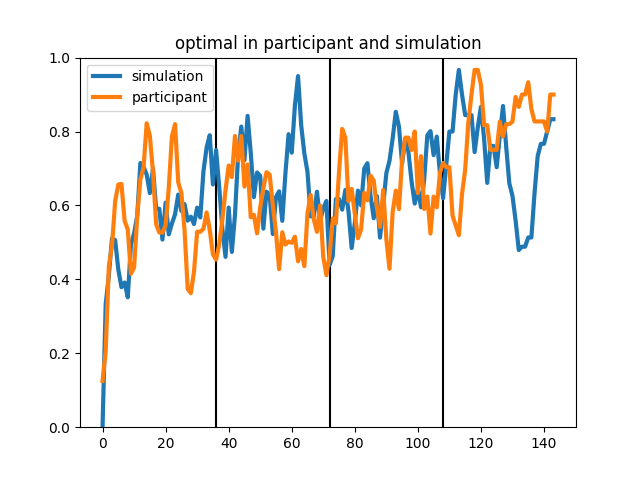
\includegraphics[width=\textwidth]{Figures/10_optimal}
\end{minipage}
}
\subfigure[Inner Optimal Percentage]{
\begin{minipage}[t]{0.48\textwidth}
\centering
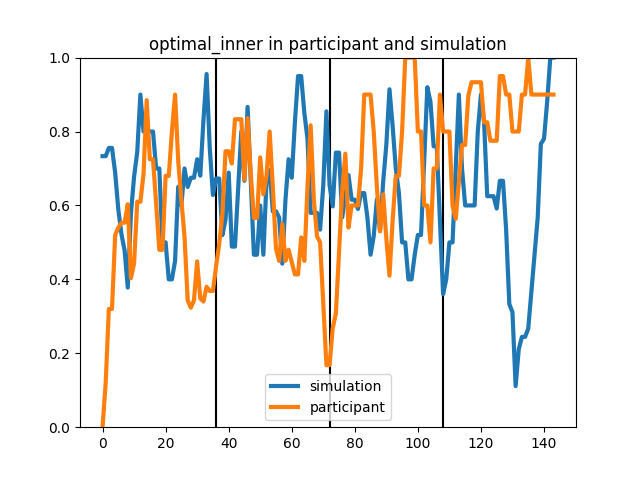
\includegraphics[width=\textwidth]{Figures/10_optimal_inner}
\end{minipage}
}
\\
\subfigure[Outer Optimal Percentage]{
\begin{minipage}[t]{0.48\textwidth}
\centering
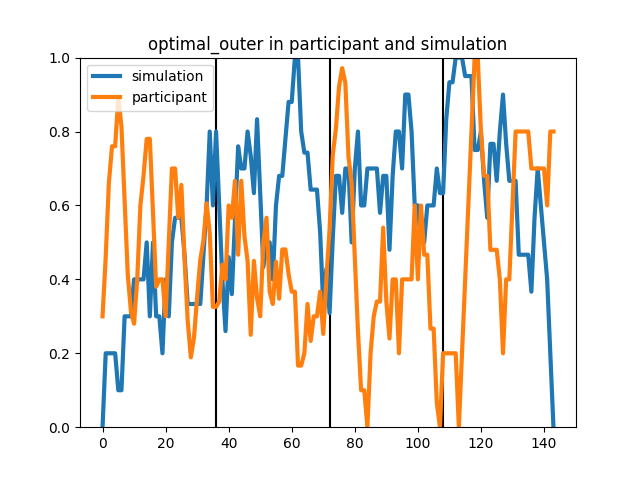
\includegraphics[width=\textwidth]{Figures/10_optimal_outer}
\end{minipage}
}
\subfigure[Last Optimal Percentage]{
\begin{minipage}[t]{0.48\textwidth}
\centering
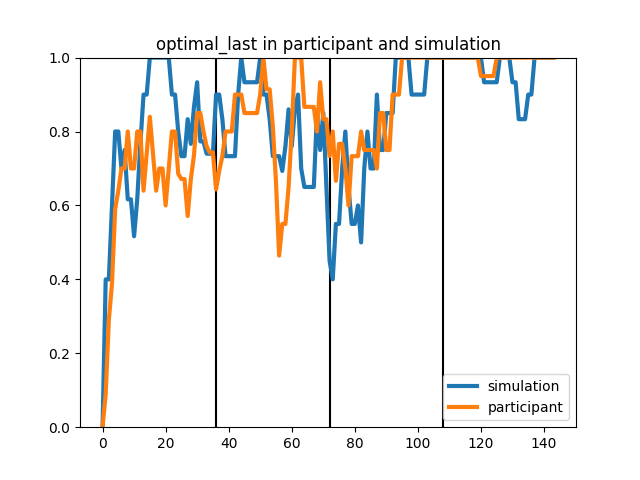
\includegraphics[width=\textwidth]{Figures/10_optimal_last}
\end{minipage}
}
\decoRule
\caption[Participant 10's data compared with Simulation]{Participant 10's data compared with Simulation}
\label{fig:Participant 10's data compared with Simulation}
\end{figure}

\paragraph{}
In this section, we want to see whether our best model, Q-learning with forget, could recreate patterns participants show in both randomized and block conditions. 
\paragraph{}
All data simulation uses the params from model fitting maximum likelihood method. Therefore, we create one simulation for each participant using their parameters under Model-Free Q-learning with forget model. It is worth noting that one simulation has strong stochasticity both due to action selection and environment transition randomness. The reason why we do not repeat the simulation several times to use the mean value is that participant's data is also only one observation. Mean values will be much smoother than participant's data because of averaging operation. 
% TODO add all simulation results in Appendix

\paragraph{}
Participant 10 and 24 is a typical example of the model simulation. Their data and simulated data are shown in Fig. \ref{fig:Participant 10's data compared with Simulation} and \ref{fig:Participant 24's data compared with Simulation}. All data patterns are reflected by simulation for participant 10 and 24. 


\begin{figure}[htb]
\centering
\subfigure[Optimal Percentage]{
\begin{minipage}[t]{0.48\textwidth}
\centering
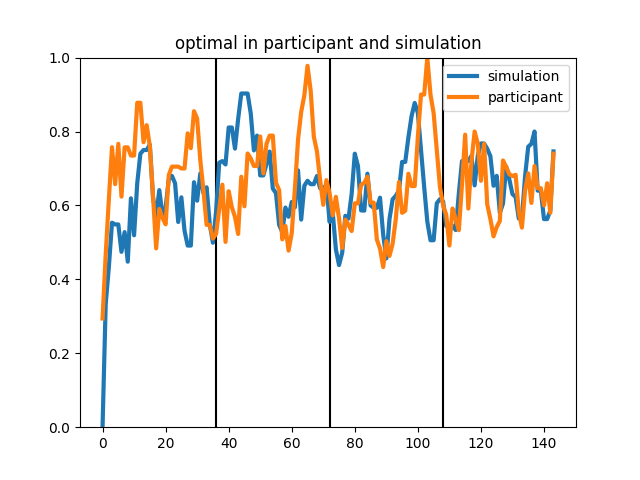
\includegraphics[width=\textwidth]{Figures/24_optimal}
\end{minipage}
}
\subfigure[Inner Optimal Percentage]{
\begin{minipage}[t]{0.48\textwidth}
\centering
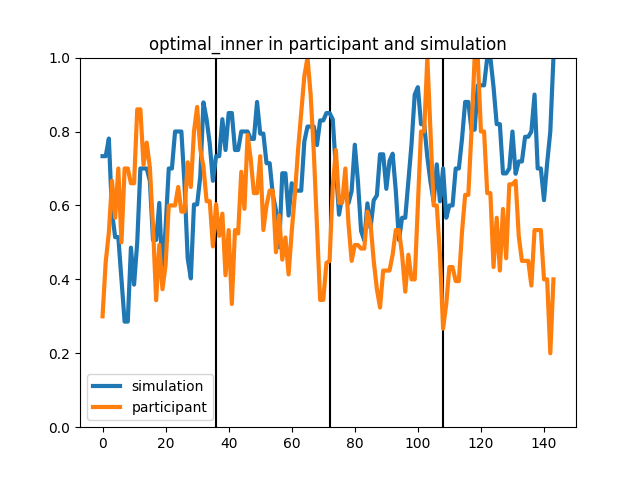
\includegraphics[width=\textwidth]{Figures/24_optimal_inner}
\end{minipage}
}
\\
\subfigure[Outer Optimal Percentage]{
\begin{minipage}[t]{0.48\textwidth}
\centering
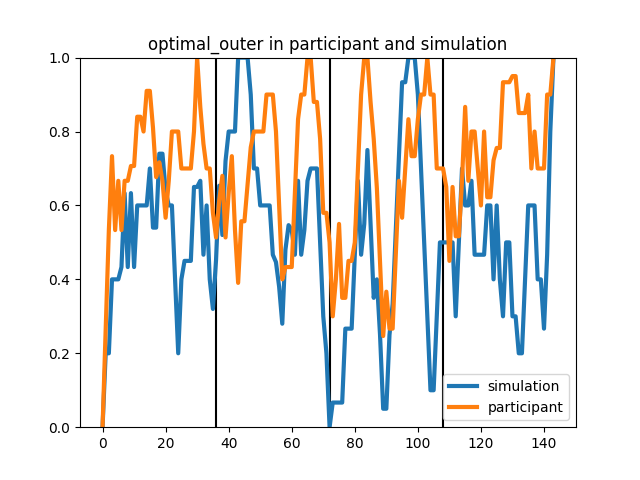
\includegraphics[width=\textwidth]{Figures/24_optimal_outer}
\end{minipage}
}
\subfigure[Last Optimal Percentage]{
\begin{minipage}[t]{0.48\textwidth}
\centering
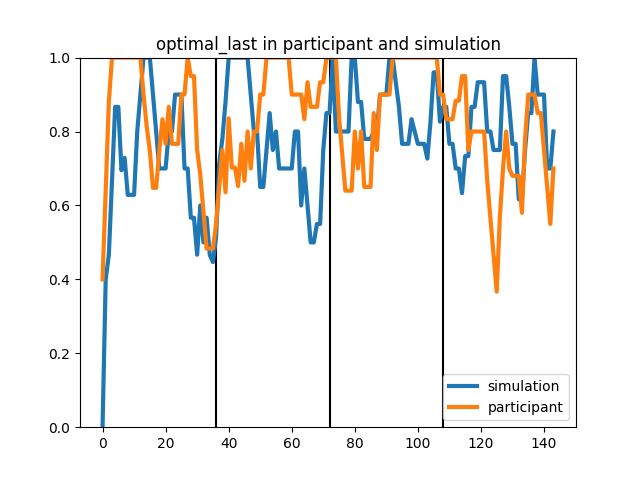
\includegraphics[width=\textwidth]{Figures/24_optimal_last}
\end{minipage}
}
\decoRule
\caption[Participant 24's data compared with Simulation]{Participant 24's data compared with Simulation}
\label{fig:Participant 24's data compared with Simulation}
\end{figure}


\paragraph{}
However, there still exist participants whose data pattern could not be captured by Model-Free model. For instance, participant 11 demonstrates a very bad performance in the beginning but soon climb to a very good performance (See Fig. \ref{fig:Participant 11's data compared with Simulation}). This seems not able to be captured by the Model-Free simulation. What's more, his best model is Hybrid model, which means the quickly increasing pattern may be a result of successfully Model-Based value estimation. 

\begin{figure}[htb]
\centering
\subfigure[Optimal Percentage]{
\begin{minipage}[t]{0.48\textwidth}
\centering
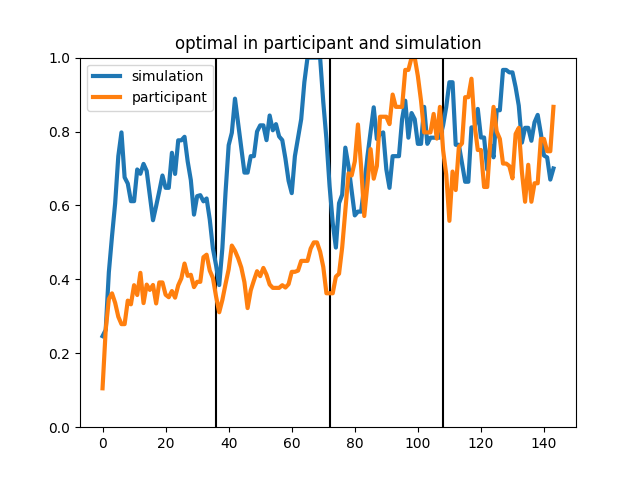
\includegraphics[width=\textwidth]{Figures/11_optimal}
\end{minipage}
}
\subfigure[Inner Optimal Percentage]{
\begin{minipage}[t]{0.48\textwidth}
\centering
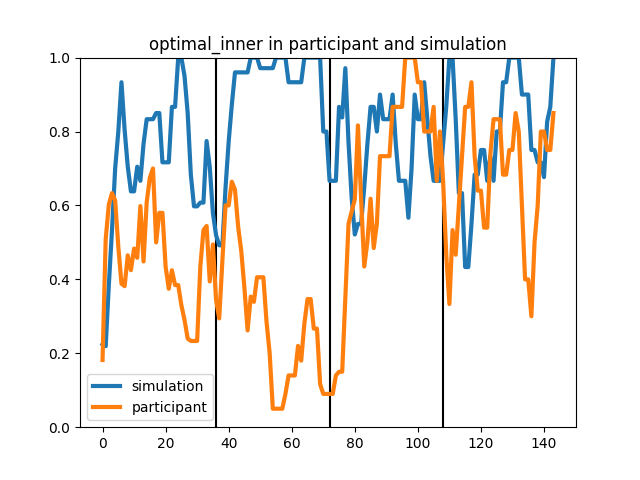
\includegraphics[width=\textwidth]{Figures/11_optimal_inner}
\end{minipage}
}
\\
\subfigure[Outer Optimal Percentage]{
\begin{minipage}[t]{0.48\textwidth}
\centering
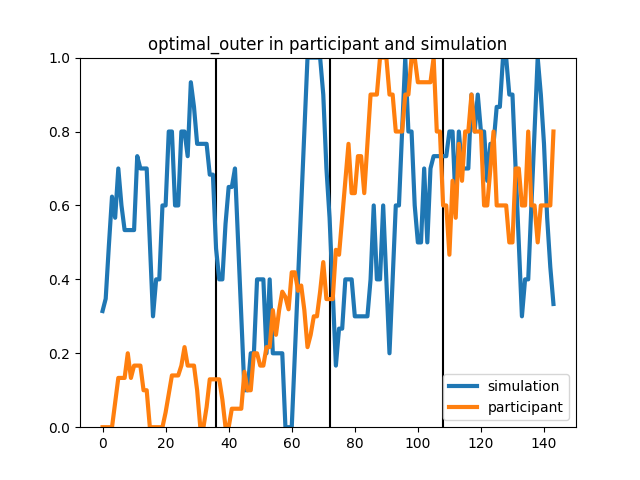
\includegraphics[width=\textwidth]{Figures/11_optimal_outer}
\end{minipage}
}
\subfigure[Last Optimal Percentage]{
\begin{minipage}[t]{0.48\textwidth}
\centering
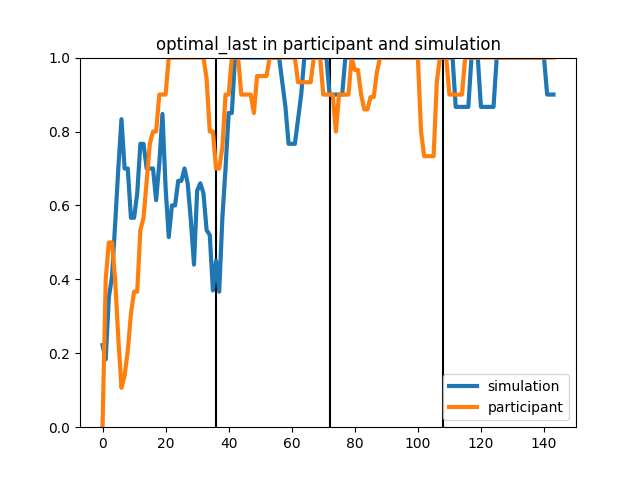
\includegraphics[width=\textwidth]{Figures/11_optimal_last}
\end{minipage}
}
\decoRule
\caption[Participant 11's data compared with Simulation]{Participant 11's data compared with Simulation}
\label{fig:Participant 11's data compared with Simulation}
\end{figure}

\paragraph{}
We also did model simulation in different parameters to see how will the data pattern change as the parameters change. Due to space limit, we put these graphs in the Appendix, while we describe some findings here. 
% add appendix ref

\paragraph{}
First of all, if the learning rate $\alpha$ or $\tau$ is close to 1, the performance will fluctuate a lot since it suffer from the stochasticity of environment transition. On the other hand, if the learning rate is close to 0, the learning will be much slower than the participants do. Therefore, a learning rate between 0.3 and 0.5 seems great in this task. 

\paragraph{}
Secondly, the softmax inverse temperature $\tau$ should never be too big or too small. If $\tau$ is close to 0, then the action selection is uniformly random regardless of value learned. If $\tau$ is bigger than 10, then the action selection will be too stable for the player, making him stuck in local optimum value. 

\paragraph{}
Finally, the forget rate. The average forget rate for participants is 0.0123, which means participants will totally forget in about 40 trials. This is reasonable because too small forget rate may result in sticking in local optimum since it can not forget the information, or transfer wrong knowledge to the following tasks. 

%----------------------------------------------------------------------------------------







 
% Chapter 6

\chapter{Chapter 6: Discussion and Conclusion} % Main chapter title

\label{Chapter 6} % For referencing the chapter elsewhere, use \ref{Chapter6} 

%----------------------------------------------------------------------------------------
\section{Discussion}
\paragraph{}
Firstly, in the model comparison results, it is clear that Model-Free method beat other models in AICc. However, there still exists several other insights. 
\paragraph{}
It is worth noting that Q-learning fits much better than SARSA, and Q-learning with forget rate fits much better than Q-learning without forget rate. It is common to add forget rate to decision making models, but it seems little RL papers ever adding forget rate to either MF or MB models. Our data has demonstrated clearly that Q value may be forgotten. 
\paragraph{}
Model-Based Centered algorithms including MB and MFHMB have worst model comparison result. The reason may be that even the MFHMB has successfully decreased computation complexity, it is still very hard to compute precisely. What's more, human's ability of probability representation is not so precise because of cognitive bias such as framework effect. These two reasons make the value estimation of Model-Based algorithms unstable and untrustworthy. Future work may design a measure in the experiment to see whether participants learn wrong probability or they learn the correct probability information but mistakenly calculate the Q value. 
\paragraph{}
The second best model is the Hybrid model. What's more interesting is that 10 of 11 participants whose Hybrid model AICc is lower than any other models are in block condition. This seems to convey us a message that in block condition people tend to use both MF and MB while in randomized condition almost all the people tend to use MF only. This may be because of working memory limit. In the block condition, participants only need to learn one task within a block while in the randomized condition participants need to learn three tasks simultaneously. The block task is easier, which means there is more space in workin memory. In this case, our brain may activate Model-Based value estimation system to help Model-Free estimation more precisely. To examine this, future work could design a side task to fulfill the free working memory to see if the Model-Based part will disappear. Another feasible way is to measure participant's working memory capacity and do correlation with Model-Based weight. 
\paragraph{}
The third best model is MBHMF model, though it has only 5 best AICc. This may indicate that the Model-Based Help Model-Free to fix mistakes. Actually the AICc of MBHMF is very close to MF model. There exists a problem that we manually set the threshold of confidently replace old action being updated. If we could relax this constraint to make the threshold a free variable, maybe MBHMF model will have a better performance. 
\paragraph{}
The rule of thumb for repeating randomly initialization is $10^n$, in which $n$ is the parameter number. Obviously we are far from the requirement. It may end up sticking in a local minimum. Future work should add more repeat times to guarantee at least a near-optimal local optimum. 
\paragraph{}
There exists another possible model: participants may never build any value or transition matrix in their brain. They just randomly pick actions until a good sequence being spotted and remembered. For example, a participant may happen to choose the optimal action sequence to reach the goal. Then he remembered the action sequence, and carry out this action sequence with 100\% probability. If they are transferred to primary sequence he will successfully win 18 tokens with probability $0.7^2=0.49$, but if not, he will randomly choose action again because he only knows how to move from start state to end state by pressing an action consequence. Future work could examine the model comparison result for these kinds of heuristic methods as well. 
%----------------------------------------------------------------------------------------


%----------------------------------------------------------------------------------------
\section{Conclusion}
In this thesis, we introduce Model-Free and Model-Based classic algorithms for Markov Decision Process. Then we design a relatively complex \enquote{labyrinth}-like environment to see how human behave in a complicated environment. The result shows participants do learn something and their performance keeps getting better along the trial set. We also fit five models to the participants' data. The result demonstrates that Q-learning is a better fit than SARSA, adding forget rate will become better fit for data, and Model-Free is the most convincing model given data but Hybrid model and Model-Based Help Model-Free model are also useful. Participant's data could not be explained totally by Model-Free model. 


%----------------------------------------------------------------------------------------

 

\begin{acknowledgements}
\addchaptertocentry{\acknowledgementname} % Add the acknowledgements to the table of contents

I would like to thank my mentor Dr. Hang Zhang for her helpful discussions and warm attitude. Doing research is never so happy! 

I also want to thank all members of CDLab for your assistance and always-smile greeting. Coding in lab is never so happy! 

I would like to thank my senior, Dian Xiong. You made me realize that everything is possible. 

I would like to thank all the people that helped me. It is because of your help that makes me go this far.

I would like to thank my parents. You gave me the most parents could ever give. 

Finally, I would like to thank my dear Zhuoting. Without you, I will never become who I am. 

\end{acknowledgements}

%----------------------------------------------------------------------------------------
%	THESIS CONTENT - APPENDICES
%----------------------------------------------------------------------------------------

\appendix % Cue to tell LaTeX that the following "chapters" are Appendices

% Include the appendices of the thesis as separate files from the Appendices folder
% Uncomment the lines as you write the Appendices

%% Appendix A

\chapter{Frequently Asked Questions} % Main appendix title

\label{AppendixA} % For referencing this appendix elsewhere, use \ref{AppendixA}

\section{How do I change the colors of links?}

The color of links can be changed to your liking using:

{\small\verb!\hypersetup{urlcolor=red}!}, or

{\small\verb!\hypersetup{citecolor=green}!}, or

{\small\verb!\hypersetup{allcolor=blue}!}.

\noindent If you want to completely hide the links, you can use:

{\small\verb!\hypersetup{allcolors=.}!}, or even better: 

{\small\verb!\hypersetup{hidelinks}!}.

\noindent If you want to have obvious links in the PDF but not the printed text, use:

{\small\verb!\hypersetup{colorlinks=false}!}.

%\include{Appendices/AppendixB}
%\include{Appendices/AppendixC}

%----------------------------------------------------------------------------------------
%	BIBLIOGRAPHY
%----------------------------------------------------------------------------------------

\printbibliography[heading=bibintoc]

%----------------------------------------------------------------------------------------

\end{document}  
